% Options for packages loaded elsewhere
\PassOptionsToPackage{unicode}{hyperref}
\PassOptionsToPackage{hyphens}{url}
\PassOptionsToPackage{dvipsnames,svgnames,x11names}{xcolor}

\documentclass[
  11pt,
  a4paper,
]{article}
\usepackage{xcolor}
\usepackage[top=26mm,bottom=24mm,left=24mm,right=24mm,headheight=15pt]{geometry}
\usepackage{amsmath,amssymb}
\setcounter{secnumdepth}{5}
\usepackage{iftex}
\ifPDFTeX
  \usepackage[T1]{fontenc}
  \usepackage[utf8]{inputenc}
  \usepackage{textcomp} % provide euro and other symbols
\else % if luatex or xetex
  \usepackage{unicode-math} % this also loads fontspec
  \defaultfontfeatures{Scale=MatchLowercase}
  \defaultfontfeatures[\rmfamily]{Ligatures=TeX,Scale=1}
\fi
\usepackage{lmodern}
\ifPDFTeX\else
  % xetex/luatex font selection
\fi
% Use upquote if available, for straight quotes in verbatim environments
\IfFileExists{upquote.sty}{\usepackage{upquote}}{}
\IfFileExists{microtype.sty}{% use microtype if available
  \usepackage[]{microtype}
  \UseMicrotypeSet[protrusion]{basicmath} % disable protrusion for tt fonts
}{}
\makeatletter
\@ifundefined{KOMAClassName}{% if non-KOMA class
  \IfFileExists{parskip.sty}{%
    \usepackage{parskip}
  }{% else
    \setlength{\parindent}{0pt}
    \setlength{\parskip}{6pt plus 2pt minus 1pt}}
}{% if KOMA class
  \KOMAoptions{parskip=half}}
\makeatother
\usepackage{longtable,booktabs,array}
\usepackage{calc} % for calculating minipage widths
% Correct order of tables after \paragraph or \subparagraph
\usepackage{etoolbox}
\makeatletter
\patchcmd\longtable{\par}{\if@noskipsec\mbox{}\fi\par}{}{}
\makeatother
% Allow footnotes in longtable head/foot
\IfFileExists{footnotehyper.sty}{\usepackage{footnotehyper}}{\usepackage{footnote}}
\makesavenoteenv{longtable}
\usepackage{graphicx}
\makeatletter
\newsavebox\pandoc@box
\newcommand*\pandocbounded[1]{% scales image to fit in text height/width
  \sbox\pandoc@box{#1}%
  \Gscale@div\@tempa{\textheight}{\dimexpr\ht\pandoc@box+\dp\pandoc@box\relax}%
  \Gscale@div\@tempb{\linewidth}{\wd\pandoc@box}%
  \ifdim\@tempb\p@<\@tempa\p@\let\@tempa\@tempb\fi% select the smaller of both
  \ifdim\@tempa\p@<\p@\scalebox{\@tempa}{\usebox\pandoc@box}%
  \else\usebox{\pandoc@box}%
  \fi%
}
% Set default figure placement to htbp
\def\fps@figure{htbp}
\makeatother
\setlength{\emergencystretch}{3em} % prevent overfull lines
\providecommand{\tightlist}{%
  \setlength{\itemsep}{0pt}\setlength{\parskip}{0pt}}
% HashAtlas group project report: typography and layout (LuaLaTeX; microtype protrusion and expansion).
% Layout follows common academic technical-report conventions: serif body, sans-serif headings,
% booktabs tables, numbered figure captions, running headers and a separate title page.

% ---------------------------------------------------------------- colours (product palette)
\definecolor{ReportInk}{HTML}{111633}
\definecolor{ReportInkTwo}{HTML}{3B3F63}
\definecolor{ReportAccent}{HTML}{6D28D9}
\definecolor{ReportAmber}{HTML}{D97706}
\definecolor{ReportRule}{HTML}{C9D3DF}
\definecolor{ReportMuted}{HTML}{5B6B7D}

% ---------------------------------------------------------------- fonts (Libertinus from TeX Live)
\setmainfont{LibertinusSerif}[Extension=.otf, UprightFont=*-Regular, BoldFont=*-Semibold,
  ItalicFont=*-Italic, BoldItalicFont=*-SemiboldItalic, Ligatures=TeX, Numbers=Lining]
\setsansfont{LibertinusSans}[Extension=.otf, UprightFont=*-Regular, BoldFont=*-Bold,
  ItalicFont=*-Italic, Numbers=Lining]
\setmonofont{LibertinusMono}[Extension=.otf, UprightFont=*-Regular, BoldFont=*-Regular, BoldFeatures={FakeBold=1.2}, Scale=0.88]
\setmathfont{LibertinusMath-Regular.otf}
\linespread{1.08}

\microtypesetup{protrusion=true,expansion=true}
\usepackage{float}
\usepackage{needspace}
\usepackage{lastpage}
\usepackage{fancyhdr}
\usepackage{titlesec}
\usepackage{tocloft}
\usepackage[font=small,labelfont={bf,sf,color=ReportInk},labelsep=period,skip=6pt]{caption}
\usepackage{enumitem}
\setlist{itemsep=2pt,topsep=4pt,leftmargin=1.4em}

% Keep figures in reading order next to the text that introduces them.
\floatplacement{figure}{H}
\setlength{\emergencystretch}{2.5em}
\setlength{\parskip}{5pt plus 1pt minus 1pt}
\widowpenalty=10000
\clubpenalty=10000

% ---------------------------------------------------------------- headings
\titleformat{\section}{\sffamily\Large\bfseries\color{ReportInk}}{\color{ReportAccent}\thesection}{0.75em}{}
\titleformat{\subsection}{\sffamily\large\bfseries\color{ReportInk}}{\color{ReportAccent}\thesubsection}{0.6em}{}
\titlespacing*{\section}{0pt}{18pt plus 4pt minus 2pt}{6pt plus 2pt}
\titlespacing*{\subsection}{0pt}{12pt plus 3pt minus 2pt}{4pt plus 1pt}

% ---------------------------------------------------------------- table of contents
\renewcommand{\cfttoctitlefont}{\sffamily\Large\bfseries\color{ReportInk}}
\renewcommand{\cftsecfont}{\sffamily\bfseries\color{ReportInk}}
\renewcommand{\cftsecpagefont}{\sffamily\bfseries\color{ReportInk}}
\renewcommand{\cftsecleader}{\cftdotfill{\cftdotsep}}
\setlength{\cftbeforesecskip}{5pt}
\renewcommand{\contentsname}{Contents}

% ---------------------------------------------------------------- tables (pandoc longtable + booktabs)
\setlength{\LTpre}{8pt}
\setlength{\LTpost}{8pt}
\renewcommand{\arraystretch}{1.18}
\setlength{\aboverulesep}{0.3ex}
\setlength{\belowrulesep}{0.5ex}
\setlength{\heavyrulewidth}{0.9pt}
\setlength{\lightrulewidth}{0.5pt}
\newenvironment{reporttable}{\par\small\sffamily}{\par}
\newenvironment{reporttablesmall}{\par\footnotesize\sffamily}{\par}

% ---------------------------------------------------------------- inline code (file paths, fields)
\newcommand{\code}[1]{{\ttfamily\color{ReportInkTwo}#1}}

% ---------------------------------------------------------------- running headers
\fancypagestyle{report}{%
  \fancyhf{}%
  \fancyhead[L]{\sffamily\footnotesize\color{ReportMuted}\ReportShortTitle}%
  \fancyhead[R]{\sffamily\footnotesize\color{ReportMuted}\nouppercase{\leftmark}}%
  \fancyfoot[C]{\sffamily\footnotesize\color{ReportMuted}\thepage\ of \pageref*{LastPage}}%
  \renewcommand{\headrulewidth}{0.4pt}%
  \renewcommand{\headrule}{{\color{ReportRule}\hrule width\headwidth height\headrulewidth}}%
}
\fancypagestyle{plain}{%
  \fancyhf{}%
  \fancyfoot[C]{\sffamily\footnotesize\color{ReportMuted}\thepage}%
  \renewcommand{\headrulewidth}{0pt}%
}
\renewcommand{\sectionmark}[1]{\markboth{\thesection\quad #1}{}}

% ---------------------------------------------------------------- title page
\newcommand{\HashAtlasTitlePage}{%
  \begin{titlepage}
    \thispagestyle{empty}
    \vspace*{30mm}
    {\sffamily\small\bfseries\color{ReportAccent}\MakeUppercase{\ReportKind}\par}
    \vspace{6mm}
    {\color{ReportRule}\rule{\linewidth}{0.8pt}\par}
    \vspace{10mm}
    {\sffamily\fontsize{28}{34}\selectfont\bfseries\color{ReportInk}\raggedright\ReportTitle\par}
    \vspace{8mm}
    {\sffamily\Large\color{ReportInkTwo}\raggedright\ReportSubtitle\par}
    \vspace{8mm}
    {\sffamily\normalsize\color{ReportInk}\raggedright\ReportTeam\par}
    \vspace{10mm}
    {\color{ReportRule}\rule{\linewidth}{0.8pt}\par}
    \vspace{6mm}
    {\sffamily\normalsize\color{ReportMuted}\raggedright\ReportDate\par}
    \vfill
  \end{titlepage}
}
\usepackage{bookmark}
\IfFileExists{xurl.sty}{\usepackage{xurl}}{} % add URL line breaks if available
\urlstyle{same}
\hypersetup{
  pdftitle={HashAtlas: Can a Small Bitcoin Miner Still Win?},
  colorlinks=true,
  linkcolor={ReportAccent},
  filecolor={Maroon},
  citecolor={Blue},
  urlcolor={ReportAccent},
  pdfcreator={LaTeX via pandoc}}

\newcommand{\ReportTitle}{HashAtlas: Can a Small Bitcoin Miner Still
Win?}
\newcommand{\ReportSubtitle}{Mining 975,494 Bitcoin blocks for miner
fingerprints, mining eras, pool families and miner decisions across
Asia}
\newcommand{\ReportDate}{CDS3004 Data Mining, Lingnan University,
2026/27 Term 1 · 14 November 2026}
\newcommand{\ReportTeam}{Team HashAtlas · LO Chi Kong, POON Tsz Chun,
SUBEDI Anukaran, YE Xiaochen, LO Ka Hung · CRN 234}
\newcommand{\ReportShortTitle}{HashAtlas · CDS3004 Group Project Report}
\newcommand{\ReportKind}{CDS3004 Data Mining · Group Project Report}

\begin{document}
\pagenumbering{roman}
\HashAtlasTitlePage

{
\hypersetup{linkcolor=ReportInk}
\setcounter{tocdepth}{1}
\tableofcontents
}
\clearpage
\pagenumbering{arabic}
\pagestyle{report}

\section{Introduction}\label{introduction}

In January 2009 anyone with a laptop could mine Bitcoin. Seventeen years
later the network computes about 1,032 exahashes per second, block
production is dominated by industrial pools, and yet every few weeks a
news story reports that a hobbyist with a single small device has ``won
the lottery'' and mined a whole block on their own. \textbf{Can a small
miner still win?} And if you live in Hong Kong or elsewhere in Asia,
what should you actually do with a mining device: join a pool, mine solo
as a lottery ticket, or switch it off?

This project answers these questions with data mining on the complete
Bitcoin block history: \textbf{975,494 blocks} from the genesis block (3
January 2009) to height 975,493 (2026-11-11), labelled with the entity
that mined each one. We combine three complementary techniques, each
matched to a question:

\begin{itemize}
\tightlist
\item
  \textbf{Classification} (decision tree, KNN, SVM): can the
  \emph{behavioural fingerprint} a miner leaves in a block (version-bit
  rolling, nonce bits, timestamps, how the block is filled) reveal who
  mined it, without reading the miner's name?
\item
  \textbf{Clustering} (K-means, four hierarchical linkages, DBSCAN): do
  the data rediscover the CPU → GPU → ASIC history of mining on their
  own, and which pools build their blocks in the same way?
\item
  \textbf{Association rules} (Apriori, implemented from scratch): which
  block properties co-occur with which miners?
\end{itemize}

The models are then \textbf{applied to new examples}: blocks with no
pool tag, blocks mined after our data freeze, and miner set-ups in 27
economies. A limited \textbf{Future Lab} explores what the 2028 halving
means for small miners, with a backtest that shows how far such
projections can be trusted. An interactive dashboard presents every
result: \url{https://cds3004.ansonlo.dev/}.

The rest of the report follows the course's six-step data-mining
workflow: problem (section 2), design (3), data (4), transformation and
selection (5-6), mining and evaluation (7-10), decisions and
interpretation (11-13), and communication, ethics and agent use (14-16).
Each member's contributions are listed in section 17.

\section{Problem definition}\label{problem-definition}

\subsection{Users and decisions}\label{users-and-decisions}

\begin{itemize}
\tightlist
\item
  \textbf{A would-be home or small-business miner in Hong Kong or Asia}
  deciding whether a device is worth running, and how (pool or solo).
\item
  \textbf{Analysts, journalists and regulators} asking how decentralised
  block production really is: a pool's \emph{name} on a block does not
  say who built the block template.
\item
  \textbf{Pool operators and researchers} who want to know which
  on-chain behaviours identify a miner (a privacy question).
\end{itemize}

\subsection{Questions and success
criteria}\label{questions-and-success-criteria}

\Needspace{11.0\baselineskip}\begin{reporttable}

\begin{longtable}[]{@{}
  >{\raggedright\arraybackslash}p{(\linewidth - 6\tabcolsep) * \real{0.0590}}
  >{\raggedright\arraybackslash}p{(\linewidth - 6\tabcolsep) * \real{0.3481}}
  >{\raggedright\arraybackslash}p{(\linewidth - 6\tabcolsep) * \real{0.2223}}
  >{\raggedright\arraybackslash}p{(\linewidth - 6\tabcolsep) * \real{0.3706}}@{}}
\toprule\noalign{}
\begin{minipage}[b]{\linewidth}\raggedright
\textbf{ID}
\end{minipage} & \begin{minipage}[b]{\linewidth}\raggedright
\textbf{Question}
\end{minipage} & \begin{minipage}[b]{\linewidth}\raggedright
\textbf{Technique}
\end{minipage} & \begin{minipage}[b]{\linewidth}\raggedright
\textbf{Success criterion (set before testing)}
\end{minipage} \\
\midrule\noalign{}
\endhead
\bottomrule\noalign{}
\endlastfoot
Q1 & From a block's fingerprint alone, which mining entity produced it?
Can solo blocks be spotted? & Classification & Clearly beat majority /
random / one-split baselines on an out-of-time test; report per-class
results and the Solo class honestly \\
Q2a & Do the data rediscover the hardware eras without being told? &
Clustering & Adjusted Rand index (ARI) against the documented eras
clearly above 0; contiguous eras \\
Q2b & Which pools build blocks alike? & Clustering + rules & Families
that are stable across linkages and consistent with the classifier's
confusions \\
Q3 & What should a miner in Hong Kong / Asia do, now and after the 2028
halving? & Decisions on new examples & Advice that follows from the
data, with explicit odds and break-even prices; future scenarios with a
published backtest error \\
\end{longtable}

\end{reporttable}

\subsection{Constraints}\label{constraints}

\begin{enumerate}
\def\labelenumi{\arabic{enumi}.}
\tightlist
\item
  \textbf{Labels are self-declared.} A block's miner is known only from
  the text a miner writes in the coinbase or from a known payout
  address. Labels can be missing (``Unknown''), copied or shared, and
  the label text itself must never be used as a model input (it would be
  leakage).
\item
  \textbf{No look-ahead.} Pools appear, merge and disappear over time,
  so evaluation must be out-of-time: train on the past, validate on the
  next period, test once on the most recent period.
\item
  \textbf{Extreme class imbalance.} Solo-mining services won only 349
  blocks in history, about 34 in the whole test period.
\item
  \textbf{Data access and scale.} Nearly a million blocks from free
  public sources with rate limits; the pipeline must resume, verify and
  record provenance. (The free Blockchair quota ran out mid-download;
  section 4 explains the switch.)
\item
  \textbf{Compute.} One workstation: SVM and nested cross-validation
  need bounded, documented samples.
\item
  \textbf{Ethics.} Public but pseudonymous data; no personal data;
  outputs must not be presented as investment advice.
\end{enumerate}

\subsection{Alternatives considered}\label{alternatives-considered}

\Needspace{12.6\baselineskip}\begin{reporttable}

\begin{longtable}[]{@{}
  >{\raggedright\arraybackslash}p{(\linewidth - 2\tabcolsep) * \real{0.4926}}
  >{\raggedright\arraybackslash}p{(\linewidth - 2\tabcolsep) * \real{0.5074}}@{}}
\toprule\noalign{}
\begin{minipage}[b]{\linewidth}\raggedright
\textbf{Alternative}
\end{minipage} & \begin{minipage}[b]{\linewidth}\raggedright
\textbf{Why not chosen}
\end{minipage} \\
\midrule\noalign{}
\endhead
\bottomrule\noalign{}
\endlastfoot
Predict the BTC price & Not a data-mining question about mining; prices
are driven by external events; widely shown to be unreliable \\
Identify pools by their coinbase tag & That is the \emph{label}; a
lookup table, not data mining, and fails exactly when a tag is absent or
shared \\
Transaction-level analysis (address clustering) & Billions of rows; out
of scope for one term and raises re-identification concerns \\
Deep learning on raw block bytes & Not interpretable, not taught in this
course, and would hide \emph{why} blocks are similar \\
Other crypto topics (Solana rug pulls, stablecoin de-pegs) & Considered
at topic selection; Bitcoin mining offered the most complete, verifiable
data across all three techniques \\
\end{longtable}

\end{reporttable}

\section{Solution design}\label{solution-design}

The design uses \textbf{three observation units}, one per question, so
that each technique works on data whose meaning fits it:

\Needspace{11.0\baselineskip}\begin{reporttable}

\begin{longtable}[]{@{}
  >{\raggedright\arraybackslash}p{(\linewidth - 6\tabcolsep) * \real{0.2271}}
  >{\raggedleft\arraybackslash}p{(\linewidth - 6\tabcolsep) * \real{0.1110}}
  >{\raggedright\arraybackslash}p{(\linewidth - 6\tabcolsep) * \real{0.4063}}
  >{\raggedright\arraybackslash}p{(\linewidth - 6\tabcolsep) * \real{0.2556}}@{}}
\toprule\noalign{}
\begin{minipage}[b]{\linewidth}\raggedright
\textbf{Unit}
\end{minipage} & \begin{minipage}[b]{\linewidth}\raggedleft
\textbf{Rows}
\end{minipage} & \begin{minipage}[b]{\linewidth}\raggedright
\textbf{Used for}
\end{minipage} & \begin{minipage}[b]{\linewidth}\raggedright
\textbf{Time meaning}
\end{minipage} \\
\midrule\noalign{}
\endhead
\bottomrule\noalign{}
\endlastfoot
Block (2019-01 → 2026-11) & 419,035 & Fingerprint classification,
association rules, anomalies & Each block is observed when mined \\
Week (2009 → 2026-10) & 926 & Era discovery (K-means, hierarchical,
DBSCAN) & Weekly aggregate of all blocks \\
Pool profile (2024 → 2026-10) & 19 & Pool families (hierarchical) & Mean
fingerprint of each pool \\
Device × economy & 212 & Miner advisor & Network state at the data
freeze \\
\end{longtable}

\end{reporttable}

\textbf{Pipeline} (\code{uv run hashatlas run-all}, 15 stages): acquire
→ clean and label → features → selection and training (frozen model
choice) → sealed test → explanations → clustering → rules → decisions →
Future Lab → figures → web data → independent verification → report →
notebook. Every stage writes its evidence to
\code{artifacts/\allowbreak{}} and is reproducible from
\code{configs/\allowbreak{}config.\allowbreak{}yaml} (random seed 3004).

\textbf{What is new in this design.} (i) Fingerprints are learnt from
\emph{behaviour only}: the label source is excluded and the version and
nonce fields are decomposed into bits because they are nominal bit
fields, not quantities. (ii) Day-relative features remove market
conditions so that only a miner's \emph{policy} remains. (iii)
Classification and clustering are joined: ``template families'' found by
hierarchical clustering on training data explain the classifier's
confusions and give a second, family-level evaluation. (iv) Decisions
are made on genuinely new blocks mined \emph{after} the analysis freeze,
and the Future Lab backtests its own method.

\section{Data collection and
preprocessing}\label{data-collection-and-preprocessing}

\subsection{Sources and acquisition}\label{sources-and-acquisition}

\Needspace{14.2\baselineskip}\begin{reporttable}

\begin{longtable}[]{@{}
  >{\raggedright\arraybackslash}p{(\linewidth - 4\tabcolsep) * \real{0.3767}}
  >{\raggedright\arraybackslash}p{(\linewidth - 4\tabcolsep) * \real{0.4130}}
  >{\raggedleft\arraybackslash}p{(\linewidth - 4\tabcolsep) * \real{0.2103}}@{}}
\toprule\noalign{}
\begin{minipage}[b]{\linewidth}\raggedright
\textbf{Source}
\end{minipage} & \begin{minipage}[b]{\linewidth}\raggedright
\textbf{Content}
\end{minipage} & \begin{minipage}[b]{\linewidth}\raggedleft
\textbf{Size}
\end{minipage} \\
\midrule\noalign{}
\endhead
\bottomrule\noalign{}
\endlastfoot
Blockchair daily block dumps & Every block 2009-2018 (one gzip TSV per
day) & 551,030 rows \\
mempool.space API: per-pool block lists + gap fill & Every block from 1
Jan 2019 (height 556,459) to 2026-11-11, with mempool.space's pool
attribution and fee-rate percentiles & 424,542 rows; 4,364 API calls \\
mempool.space mining-pool definitions (open source) & 172 pools,
coinbase tags and payout addresses & 1 JSON \\
mempool.space solo-service block lists & 349 blocks of 6 solo services &
1 JSON \\
blockchain.com charts & Daily hash rate, price, miner revenue, fees
since 2009 & 6,519 days \\
GlobalPetrolPrices (dated snapshot) & Household and business electricity
prices, USD/kWh & 144 countries \\
\end{longtable}

\end{reporttable}

\textbf{Loading a large dataset.} The \textasciitilde4,000 daily dump
files are read in parallel with explicit dtypes and only the needed
columns, concatenated (about one million rows), de-duplicated by height
and stored as Parquet. Every raw file has a SHA-256 hash in
\code{artifacts/\allowbreak{}source\_\allowbreak{}manifest.\allowbreak{}json};
downloads resume and retry with back-off. Mid-way through, the free
Blockchair dump quota was exhausted (HTTP 402), so from 2019 onwards
every block was fetched from mempool.space per pool (100 blocks per
call), and any isolated height missing from either source was filled
individually. The final table has \textbf{no missing and no duplicate
heights} (0 to 975,493).

\subsection{Attribute types}\label{attribute-types}

Conceptual measurement scale is recorded separately from storage type
(Lecture 2). Key decisions:

\begin{itemize}
\tightlist
\item
  \code{version} and \code{nonce} are stored as integers but are
  \textbf{nominal bit fields}: bit 13 being set says something about the
  miner's software; ``version = 0x2FFFE000 is larger than 0x20000000''
  says nothing. They are decomposed into bits.
\item
  \code{height} is ordinal (a position), \code{time} is interval, counts
  and sizes are ratio-scaled, \code{miner} is nominal.
\item
  The full data dictionary with scale, discrete/continuous status and
  role is in
  \code{artifacts/\allowbreak{}data\_\allowbreak{}dictionary.\allowbreak{}csv}
  (and the dashboard's Methods page).
\end{itemize}

\subsection{Data quality: problems found and how they were
handled}\label{data-quality-problems-found-and-how-they-were-handled}

\Needspace{15.8\baselineskip}\begin{reporttable}

\begin{longtable}[]{@{}
  >{\raggedright\arraybackslash}p{(\linewidth - 4\tabcolsep) * \real{0.2055}}
  >{\raggedright\arraybackslash}p{(\linewidth - 4\tabcolsep) * \real{0.3545}}
  >{\raggedright\arraybackslash}p{(\linewidth - 4\tabcolsep) * \real{0.4399}}@{}}
\toprule\noalign{}
\begin{minipage}[b]{\linewidth}\raggedright
\textbf{Issue}
\end{minipage} & \begin{minipage}[b]{\linewidth}\raggedright
\textbf{Finding}
\end{minipage} & \begin{minipage}[b]{\linewidth}\raggedright
\textbf{Handling}
\end{minipage} \\
\midrule\noalign{}
\endhead
\bottomrule\noalign{}
\endlastfoot
Missing values & Total input/output value and coin-days destroyed are
not provided by mempool.space (424,464 rows) & Not used (not needed);
fee rate recomputed where missing \\
Out-of-order timestamps & 16,279 blocks (1.67\%) have an earlier
timestamp than their predecessor & \textbf{Kept}: consensus allows it;
it reflects miner clocks and is a candidate fingerprint, not an error \\
Empty blocks & 89,947 coinbase-only blocks & Kept; genuine miner
behaviour (an empty-block flag is a feature) \\
Under-claimed rewards & 1,124 blocks claimed less than subsidy + fees
(mostly 2011-2013 pool software); none claimed more & Kept; the subsidy
is taken from the schedule, revenue from what was actually claimed \\
Difficulty consistency & Difficulty bits change only at retarget heights
(0 violations) & Verified \\
Unattributed blocks & ``Unknown'' miner: 100\% of blocks in 2010, 0.09\%
in 2024 & A genuine state, not a missing value: excluded from training,
used as the application set (section 11) \\
Heavy tails / noise & Fees, transaction counts and sizes span orders of
magnitude & log1p transforms; extremes are real (e.g.~inscription-heavy
blocks), so none deleted \\
\end{longtable}

\end{reporttable}

\begin{figure}
\centering
\pandocbounded{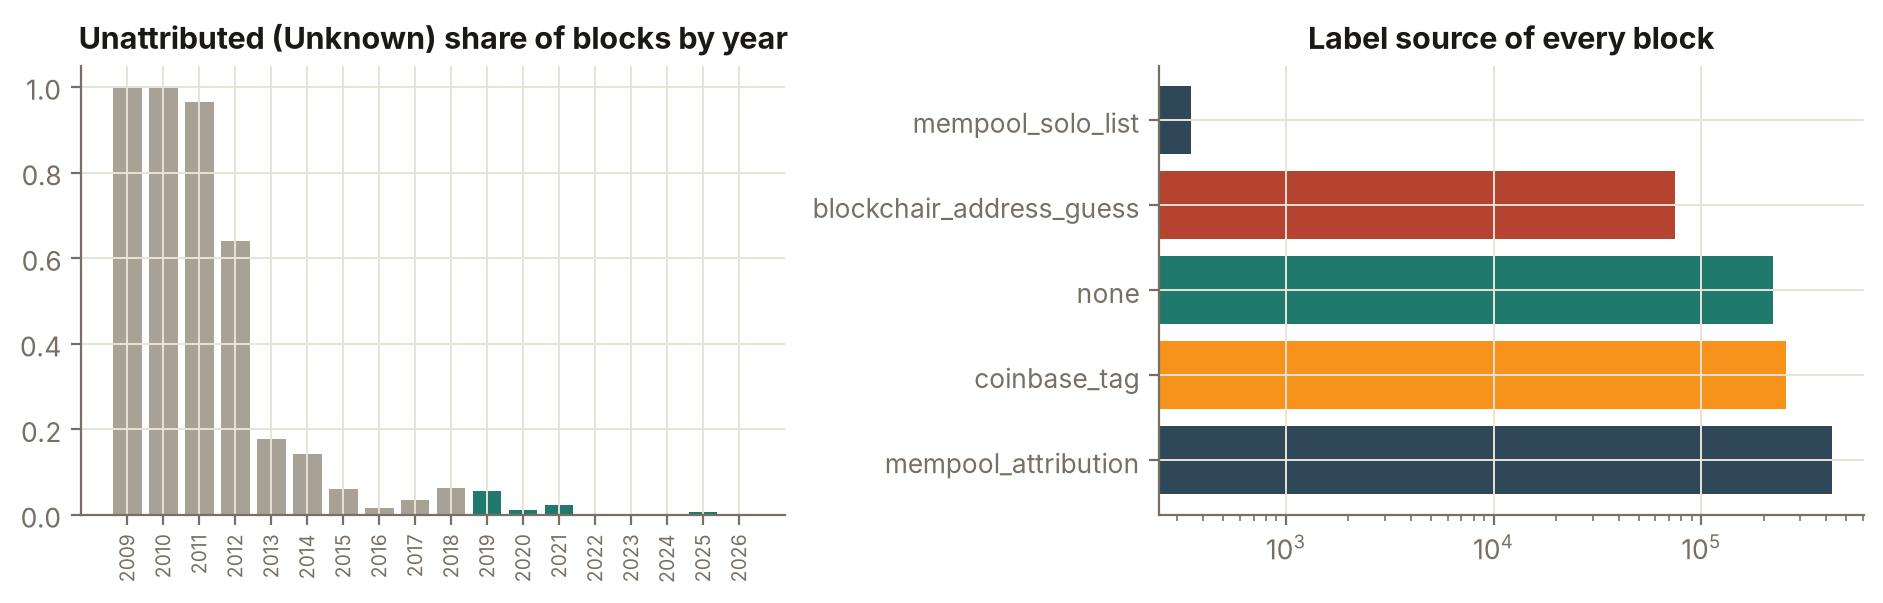
\includegraphics[keepaspectratio,alt={Unattributed share of blocks by year, and the source of every label.}]{figures/f04_label_quality.png}}
\caption{Unattributed share of blocks by year, and the source of every
label.}
\end{figure}

\subsection{Label quality audit}\label{label-quality-audit}

Labels for 2019+ come from mempool.space's attribution (coinbase tags
\emph{and} payout addresses, curated). Labels for 2009-2018 come from
our own transparent labeller: the first matching coinbase tag from the
same open definition file, then Blockchair's address-based guess. To
measure how good our labeller is, we \textbf{re-applied it to all
424,464 mempool.space-labelled blocks} and compared:

\begin{itemize}
\tightlist
\item
  when our labeller finds a tag, it agrees with mempool.space
  \textbf{99.95\%} of the time;
\item
  it finds a tag for 92.6\% of blocks; the rest are mainly pools
  identified only by payout address (largest: F2Pool, 11,426 blocks),
  which our labeller marks Unknown rather than guessing;
\item
  overall agreement 94.2\%. Early-era labels are therefore precise but
  somewhat incomplete, which only affects descriptive statistics
  (section 9), not the 2019+ models.
\end{itemize}

\begin{figure}
\centering
\pandocbounded{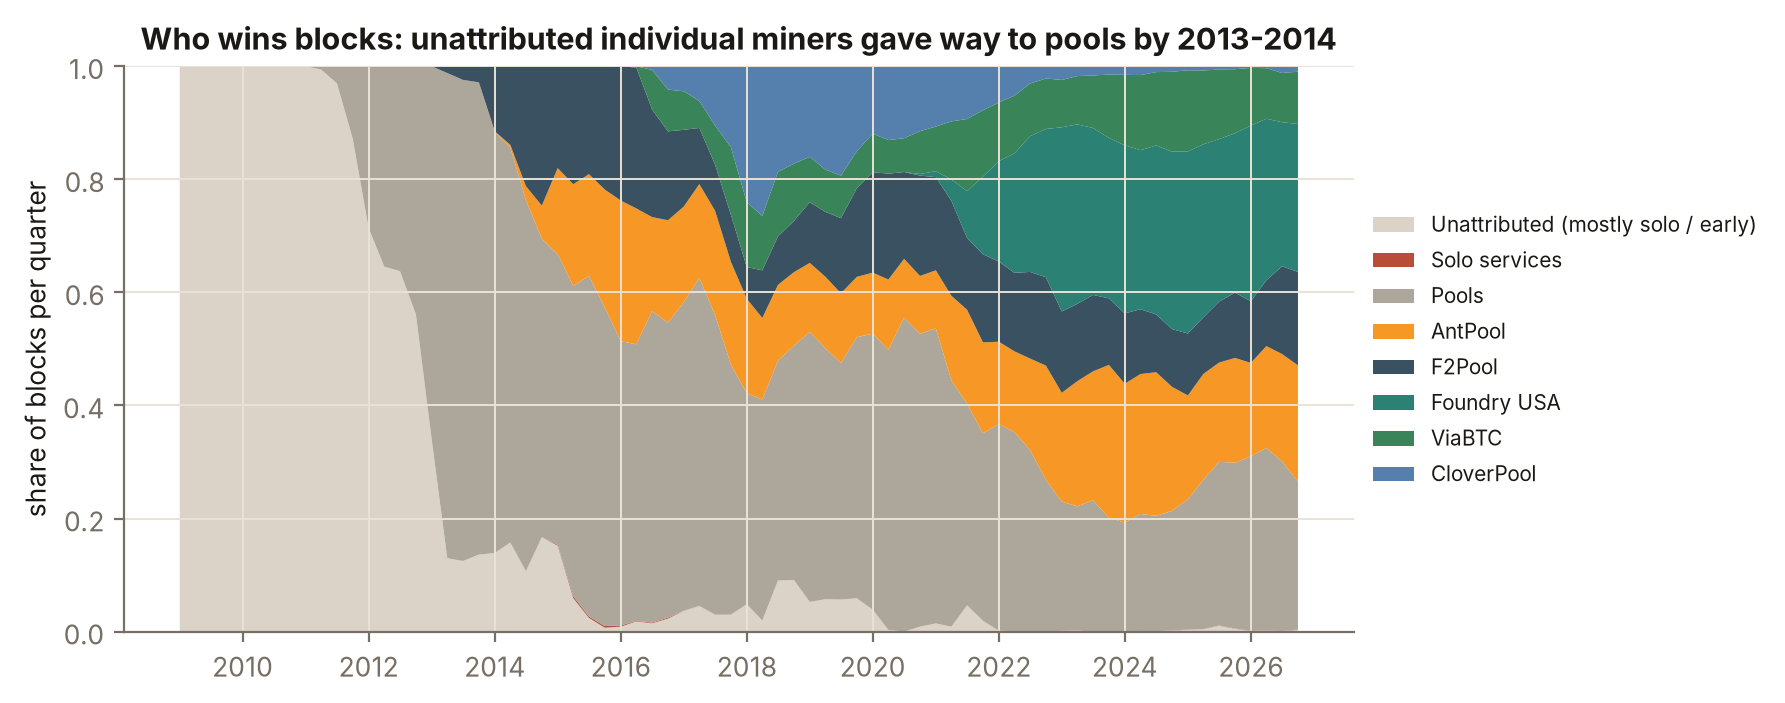
\includegraphics[keepaspectratio,alt={Share of blocks per quarter: unattributed early miners gave way to pools by 2013-2014.}]{figures/f02_who_mines.png}}
\caption{Share of blocks per quarter: unattributed early miners gave way
to pools by 2013-2014.}
\end{figure}

\section{Feature transformation}\label{feature-transformation}

All transformations are fitted on training data only where they have
parameters (scaling, bins).

\Needspace{17.4\baselineskip}\begin{reporttable}

\begin{longtable}[]{@{}
  >{\raggedright\arraybackslash}p{(\linewidth - 4\tabcolsep) * \real{0.2791}}
  >{\raggedright\arraybackslash}p{(\linewidth - 4\tabcolsep) * \real{0.3645}}
  >{\raggedright\arraybackslash}p{(\linewidth - 4\tabcolsep) * \real{0.3565}}@{}}
\toprule\noalign{}
\begin{minipage}[b]{\linewidth}\raggedright
\textbf{Transformation}
\end{minipage} & \begin{minipage}[b]{\linewidth}\raggedright
\textbf{Applied to}
\end{minipage} & \begin{minipage}[b]{\linewidth}\raggedright
\textbf{Why}
\end{minipage} \\
\midrule\noalign{}
\endhead
\bottomrule\noalign{}
\endlastfoot
Bit decomposition & version bits 13-28 (BIP320 general-purpose bits used
by ASICBoost rolling), count of rolled bits, BIP9 top bits, signal bits;
nonce bits 0-31 & Nominal bit fields: each bit is a binary attribute;
distances on the raw integer would be meaningless \\
log1p & transaction count, fees, fee rate, minimum fee rate, mean
transaction size & Heavy right tails \\
Ratios and shares & fullness = weight / 4,000,000; witness share; fee
share of reward; log(outputs) − log(inputs) & Comparable across eras and
block sizes \\
\textbf{Day-relative policy} & fee rate, minimum/median fee, fee
percentiles, transaction count, fullness, each minus the median of all
blocks that day & Removes market conditions (busy vs quiet days) so that
only the miner's template policy remains \\
Cyclic encoding & hour of day (sin, cos) & Included as a
\textbf{deliberately irrelevant control}: blocks are found at random
times, so selection should remove it \\
Standardisation & all features, inside the KNN and SVM pipelines (fitted
per training fold) & Distance-based methods need comparable scales \\
Weekly aggregation & 9 era features (log hash rate, 30-day growth, empty
share, transactions per block, fullness, fee share, unattributed share,
HHI concentration, log BTC earned per TH/s) & Removes daily noise for
era clustering \\
Frontier hardware and break-even price & best available J/TH by date
(CPU → S21 XP); break-even USD/kWh = hash price ÷ energy per TH-day &
Turns network data into the economics a miner faces \\
\end{longtable}

\end{reporttable}

\textbf{Excluded by design (leakage control):} coinbase text, payout
address, Blockchair's miner guess (all label sources), block height and
calendar time (they only encode which pools were large \emph{when}), and
network difficulty (identical for every miner in the same period). An
automated check confirms none of them reached the model (section 15).

\section{Feature selection}\label{feature-selection}

Feature selection used \textbf{training data only} (2019-2023,
month-stratified sample of 60,001 blocks) and four complementary
methods, from filter to wrapper:

\Needspace{12.6\baselineskip}\begin{reporttable}

\begin{longtable}[]{@{}
  >{\raggedleft\arraybackslash}p{(\linewidth - 6\tabcolsep) * \real{0.0720}}
  >{\raggedright\arraybackslash}p{(\linewidth - 6\tabcolsep) * \real{0.4076}}
  >{\raggedright\arraybackslash}p{(\linewidth - 6\tabcolsep) * \real{0.3405}}
  >{\raggedleft\arraybackslash}p{(\linewidth - 6\tabcolsep) * \real{0.1799}}@{}}
\toprule\noalign{}
\begin{minipage}[b]{\linewidth}\raggedleft
\textbf{Step}
\end{minipage} & \begin{minipage}[b]{\linewidth}\raggedright
\textbf{Method}
\end{minipage} & \begin{minipage}[b]{\linewidth}\raggedright
\textbf{Removed}
\end{minipage} & \begin{minipage}[b]{\linewidth}\raggedleft
\textbf{Remaining}
\end{minipage} \\
\midrule\noalign{}
\endhead
\bottomrule\noalign{}
\endlastfoot
0 & Candidate fingerprint features & -- & 77 \\
1 & Variance filter (min-max scaled variance \textless{} 1e-4) & 0 &
77 \\
2 & Mutual information vs.~10 random noise probes (cutoff 0.00019) & 19
& 58 \\
3 & Redundancy: & Spearman ρ & \textgreater{} 0.90, keep higher MI \\
4 & Wrapper: drop-one-group ablation (tree, month-grouped CV) & fee
ladder (percentiles), hour of day (control) & 51 \\
\end{longtable}

\end{reporttable}

Findings worth noting:

\begin{itemize}
\tightlist
\item
  \textbf{Timing carries no miner signal.} Both timestamp features
  (offset from the median of the previous 11 blocks and interval since
  the previous block) scored below the noise probes and were removed,
  consistent with block discovery being a random (Poisson) process for
  every miner.
\item
  \textbf{The control feature was caught}: the hour-of-day encodings
  were removed (one by mutual information, the other by the ablation),
  as designed.
\item
  Most nonce bits are noise; a few low-order bits survive (some mining
  hardware searches the nonce space in a structured way).
\item
  Redundant pair removed: log\_fee\_total vs log\_fee\_per\_kwu (ρ =
  0.929), rel\_fee\_p10 vs rel\_fee\_p25 (ρ = 0.912).
\end{itemize}

\Needspace{14.2\baselineskip}\begin{reporttable}

\begin{longtable}[]{@{}
  >{\raggedright\arraybackslash}p{(\linewidth - 6\tabcolsep) * \real{0.2924}}
  >{\raggedleft\arraybackslash}p{(\linewidth - 6\tabcolsep) * \real{0.1362}}
  >{\raggedleft\arraybackslash}p{(\linewidth - 6\tabcolsep) * \real{0.4605}}
  >{\raggedleft\arraybackslash}p{(\linewidth - 6\tabcolsep) * \real{0.1110}}@{}}
\toprule\noalign{}
\begin{minipage}[b]{\linewidth}\raggedright
\textbf{Feature group}
\end{minipage} & \begin{minipage}[b]{\linewidth}\raggedleft
\textbf{Features kept}
\end{minipage} & \begin{minipage}[b]{\linewidth}\raggedleft
\textbf{CV macro-F1 without the group}
\end{minipage} & \begin{minipage}[b]{\linewidth}\raggedleft
\textbf{Change}
\end{minipage} \\
\midrule\noalign{}
\endhead
\bottomrule\noalign{}
\endlastfoot
version bits & 20 & 0.3024 & -0.0400 \\
nonce bits & 17 & 0.3421 & -0.0003 \\
body composition & 10 & 0.2834 & -0.0590 \\
day-relative policy & 4 & 0.3389 & -0.0035 \\
fee ladder (percentiles) & 4 & 0.3434 & +0.0009 \\
hour of day (control) & 1 & 0.3426 & +0.0002 \\
\end{longtable}

\end{reporttable}

Version bits and body composition carry most of the signal. The final
model uses \textbf{51 features}.

\begin{figure}
\centering
\pandocbounded{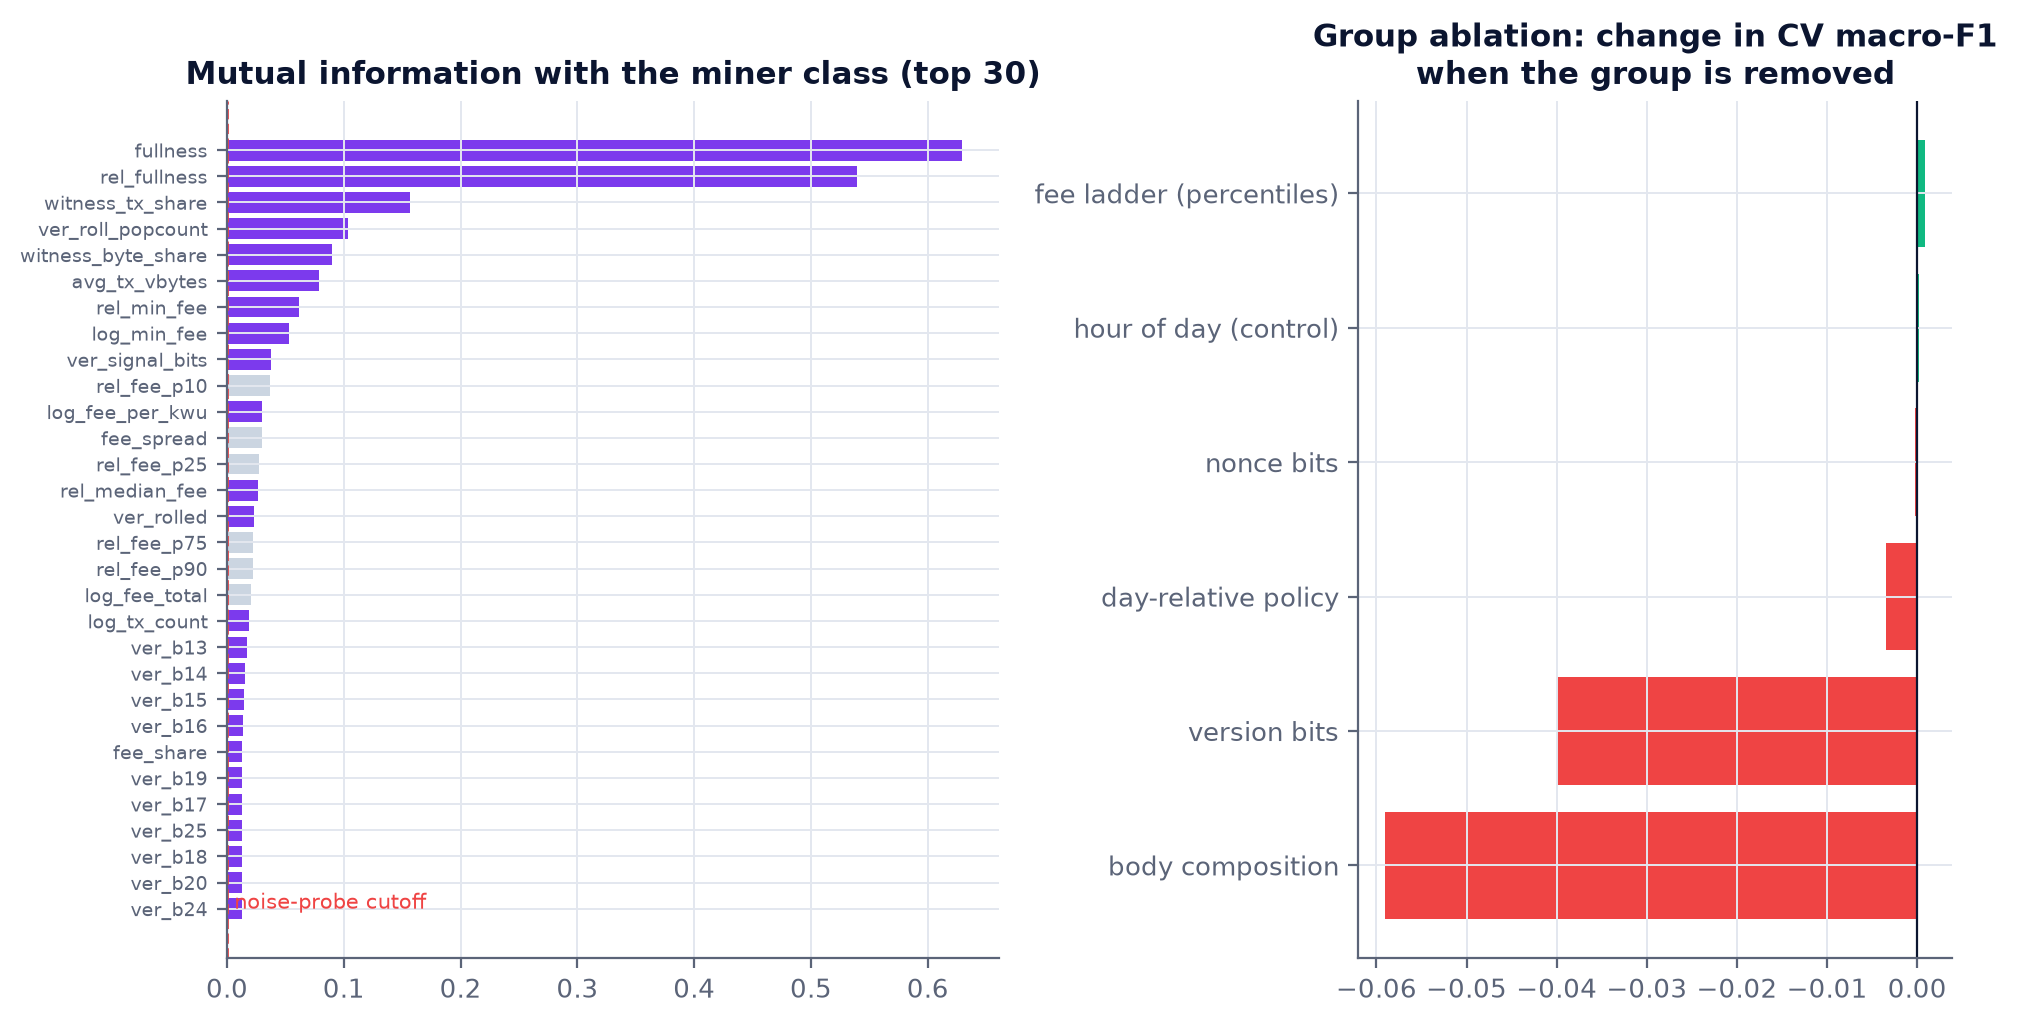
\includegraphics[keepaspectratio,alt={Left: mutual information of the top 30 candidates (violet = kept) against the noise-probe cutoff. Right: change in CV macro-F1 when a feature group is removed.}]{figures/f05_feature_selection.png}}
\caption{Left: mutual information of the top 30 candidates (violet =
kept) against the noise-probe cutoff. Right: change in CV macro-F1 when
a feature group is removed.}
\end{figure}

\section{Model learning procedure}\label{model-learning-procedure}

\subsection{Target and data splits}\label{target-and-data-splits}

The target is the mining entity of a block: the 10 pools that mined at
least 2\% of training-period blocks, an \textbf{Other pools} class, and
a \textbf{Solo} class (the six solo-mining services). Unknown blocks are
never used for fitting.

\Needspace{11.0\baselineskip}\begin{reporttable}

\begin{longtable}[]{@{}
  >{\raggedright\arraybackslash}p{(\linewidth - 8\tabcolsep) * \real{0.1500}}
  >{\raggedright\arraybackslash}p{(\linewidth - 8\tabcolsep) * \real{0.2176}}
  >{\raggedleft\arraybackslash}p{(\linewidth - 8\tabcolsep) * \real{0.1416}}
  >{\raggedleft\arraybackslash}p{(\linewidth - 8\tabcolsep) * \real{0.0720}}
  >{\raggedright\arraybackslash}p{(\linewidth - 8\tabcolsep) * \real{0.4188}}@{}}
\toprule\noalign{}
\begin{minipage}[b]{\linewidth}\raggedright
\textbf{Split}
\end{minipage} & \begin{minipage}[b]{\linewidth}\raggedright
\textbf{Period}
\end{minipage} & \begin{minipage}[b]{\linewidth}\raggedleft
\textbf{Labelled blocks}
\end{minipage} & \begin{minipage}[b]{\linewidth}\raggedleft
\textbf{Solo}
\end{minipage} & \begin{minipage}[b]{\linewidth}\raggedright
\textbf{Role}
\end{minipage} \\
\midrule\noalign{}
\endhead
\bottomrule\noalign{}
\endlastfoot
Train & 2019-01-01 → 2023-12-31 & 262,327 & 28 & feature selection,
hyper-parameters (CV), nested CV \\
Validation & 2024-01-01 → 2025-03-31 & 66,449 & 23 & model-family
choice, Solo threshold (out of time) \\
Test (sealed) & 2025-04-01 → 2026-10-31 & 83,387 & 34 & scored once,
after the choice was frozen \\
New & 2026-11-01 → 2026-11-11 & 1,446 & 3 & mined after the data freeze:
decision demo \\
\end{longtable}

\end{reporttable}

\textbf{Cross-validation adapted to time.} Shuffled k-fold would put
blocks from the same day in both training and validation folds and
overstate accuracy. Folds are therefore \textbf{grouped by calendar
month} (5-fold GroupKFold). The training sample keeps every Solo block
and a month-stratified proportional sample of the rest (representative
sampling, Lecture 3).

\subsection{Algorithms and
hyper-parameters}\label{algorithms-and-hyper-parameters}

\Needspace{11.0\baselineskip}\begin{reporttable}

\begin{longtable}[]{@{}
  >{\raggedright\arraybackslash}p{(\linewidth - 8\tabcolsep) * \real{0.1247}}
  >{\raggedright\arraybackslash}p{(\linewidth - 8\tabcolsep) * \real{0.2744}}
  >{\raggedright\arraybackslash}p{(\linewidth - 8\tabcolsep) * \real{0.3427}}
  >{\raggedleft\arraybackslash}p{(\linewidth - 8\tabcolsep) * \real{0.1322}}
  >{\raggedleft\arraybackslash}p{(\linewidth - 8\tabcolsep) * \real{0.1260}}@{}}
\toprule\noalign{}
\begin{minipage}[b]{\linewidth}\raggedright
\textbf{Model}
\end{minipage} & \begin{minipage}[b]{\linewidth}\raggedright
\textbf{Grid searched}
\end{minipage} & \begin{minipage}[b]{\linewidth}\raggedright
\textbf{Chosen}
\end{minipage} & \begin{minipage}[b]{\linewidth}\raggedleft
\textbf{CV macro-F1 (± SE)}
\end{minipage} & \begin{minipage}[b]{\linewidth}\raggedleft
\textbf{Train macro-F1}
\end{minipage} \\
\midrule\noalign{}
\endhead
\bottomrule\noalign{}
\endlastfoot
Decision tree & criterion \{gini, entropy\} × max\_depth \{3\ldots16,
none\} × min\_samples\_leaf \{5, 20, 50\} × class\_weight \{none,
balanced\} & class\_weight=balanced, criterion=gini, max\_depth=12,
min\_samples\_leaf=5 & 0.377 ± 0.009 & 0.458 \\
KNN & k \{5, 15, 41\} × weights \{uniform, distance\} × metric
\{Manhattan, Euclidean\}; standardised & metric=euclidean,
n\_neighbors=41, weights=distance & 0.156 ± 0.003 & 1.000 \\
Linear SVM & C \{0.01, 0.1, 1, 10\}; balanced classes; 8,000-row sample
& C=10.0 & 0.144 ± 0.006 & 0.176 \\
RBF SVM & C \{1, 10\} × γ \{scale, 0.03\}; balanced; 8,000-row sample &
C=1.0, gamma=0.03 & 0.180 ± 0.003 & 0.539 \\
\end{longtable}

\end{reporttable}

The SVMs are trained on a bounded sample because kernel SVM cost grows
roughly quadratically with rows; all models are scored on identical
validation and test blocks. \textbf{Nested cross-validation} (outer 5 ×
inner 3, month-grouped) estimates the \emph{whole} tree-tuning procedure
without optimistic bias: macro-F1 \textbf{0.378 ± 0.021} (SD over outer
folds), close to the inner CV score, so the grid search did not overfit
its own folds.

\begin{figure}
\centering
\pandocbounded{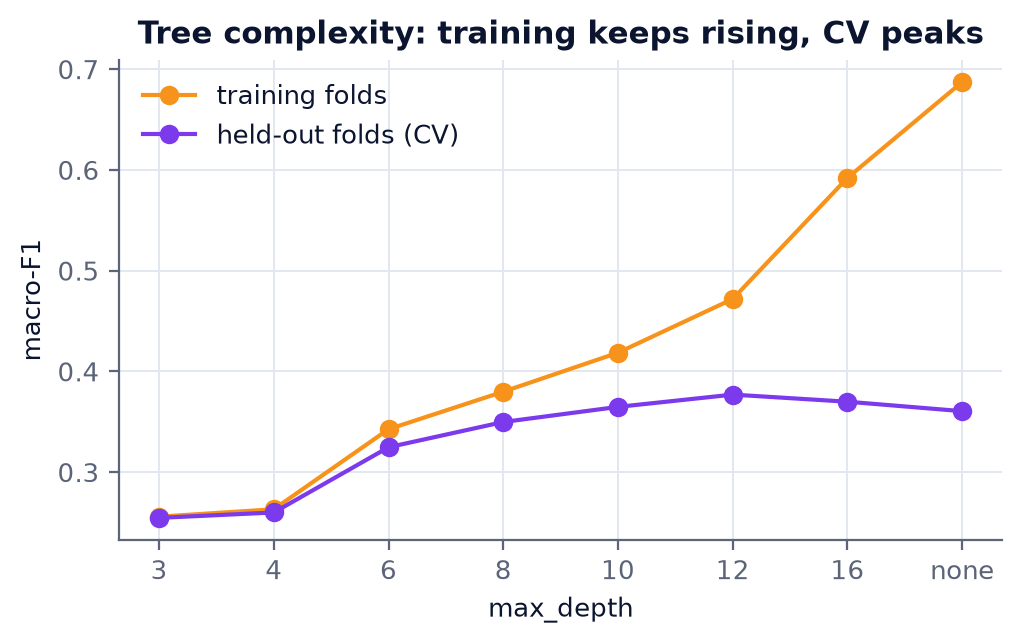
\includegraphics[keepaspectratio,alt={Tree complexity: training macro-F1 keeps rising with depth while held-out CV levels off, the classic overfitting signature.}]{figures/f06_tree_complexity.png}}
\caption{Tree complexity: training macro-F1 keeps rising with depth
while held-out CV levels off, the classic overfitting signature.}
\end{figure}

\subsection{How the tree splits (worked
example)}\label{how-the-tree-splits-worked-example}

The root of the training tree tests \textbf{\code{fullness} ≤ 0.998}.
Recomputed by hand on 60,001 training blocks: parent Gini 0.8890; left
child (50,210 blocks) Gini 0.8825; right child (9,791 blocks) Gini
0.4306; weighted child impurity (n\textsubscript{L}G\textsubscript{L} +
n\textsubscript{R}G\textsubscript{R})/n = 0.8088; \textbf{Gini reduction
0.0802} (entropy information gain 0.3933). Gini and entropy reached CV
scores of 0.377 and 0.373; the chosen criterion was gini. The fitted
tree is exported in full to the dashboard, where any test block can be
traced root-to-leaf.

\begin{figure}
\centering
\pandocbounded{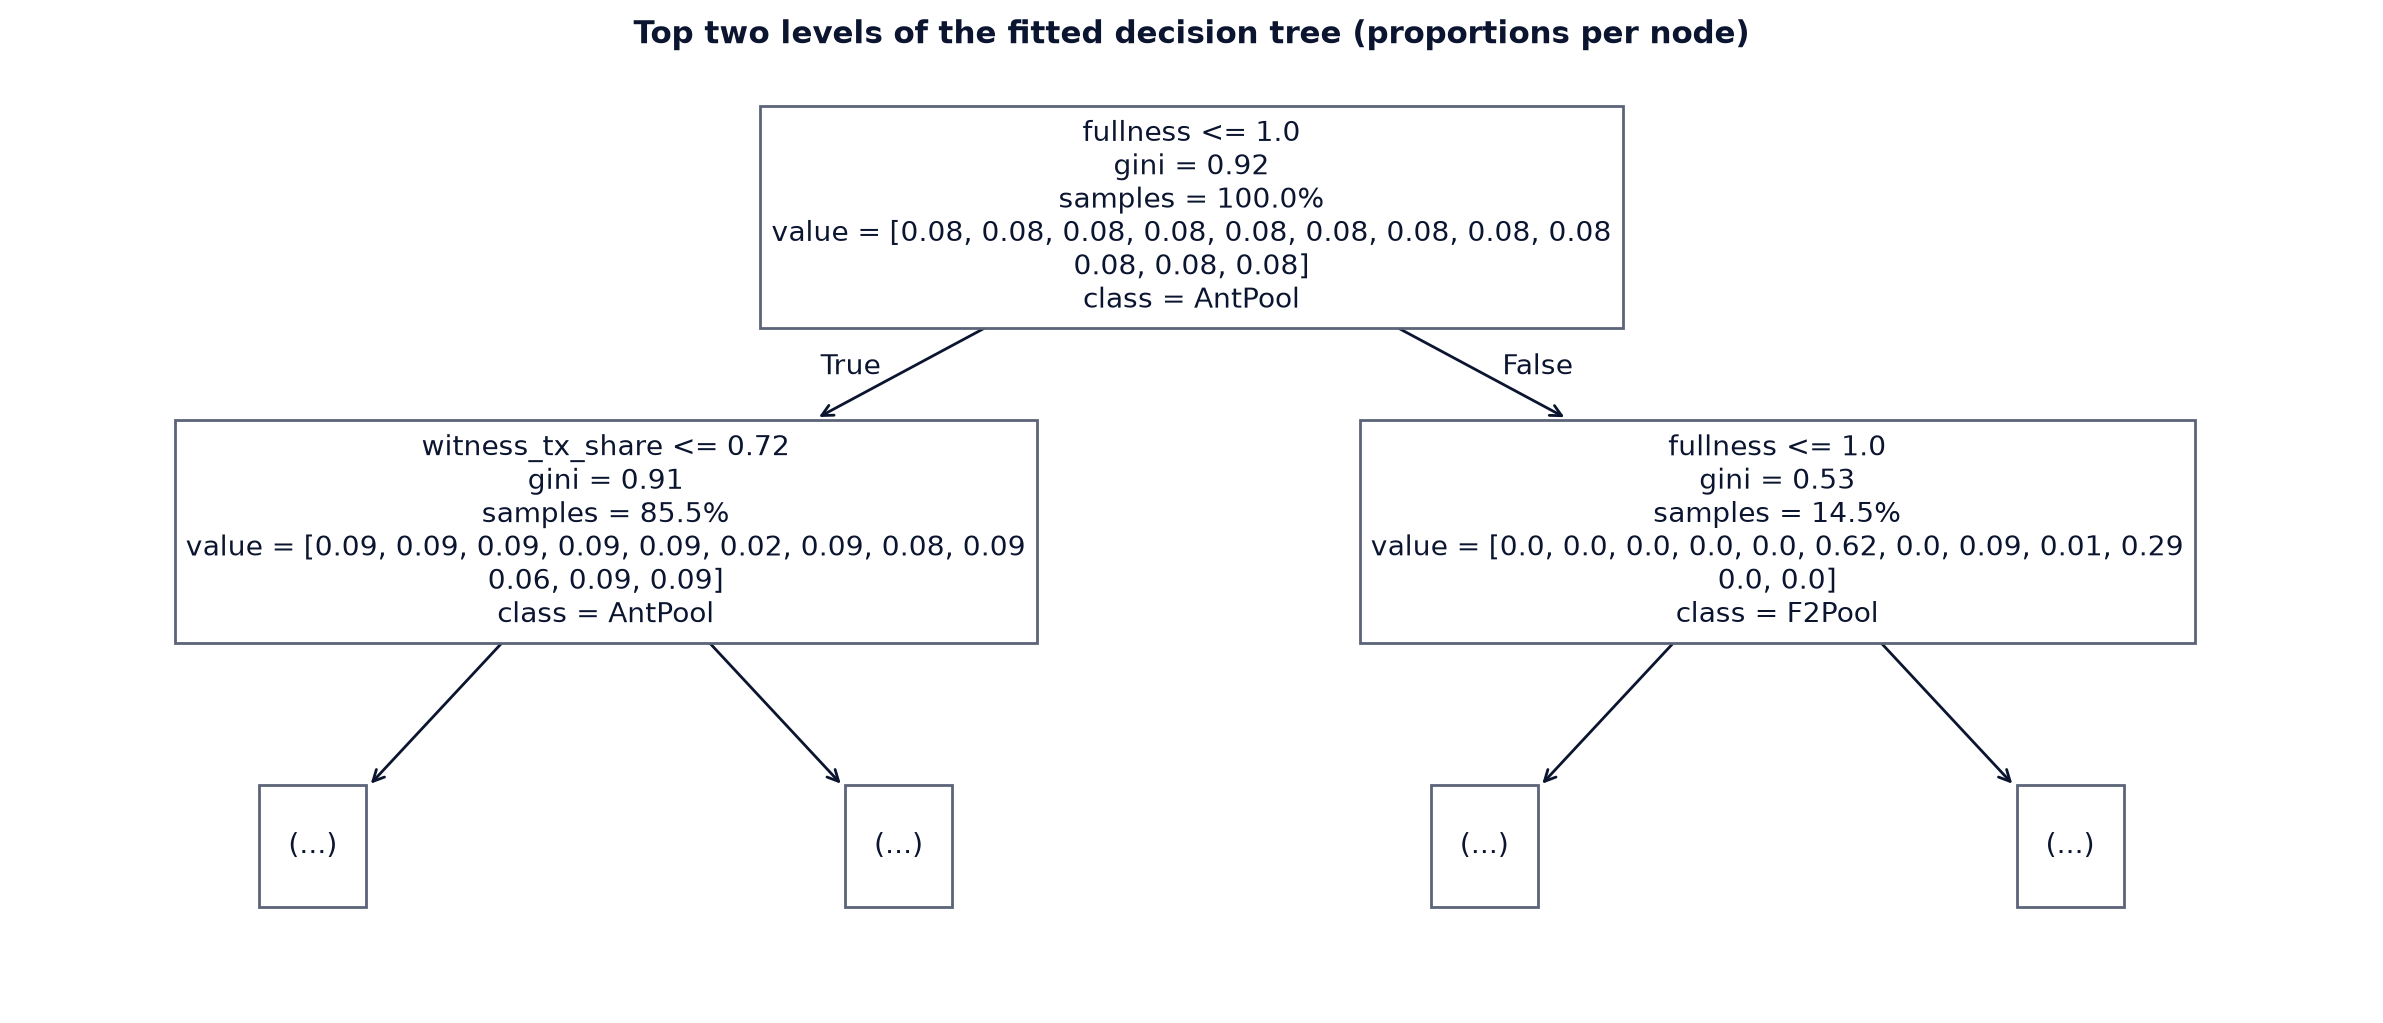
\includegraphics[keepaspectratio,alt={Top two levels of the fitted decision tree (class proportions per node); the full tree is in the dashboard.}]{figures/f11_tree_top.png}}
\caption{Top two levels of the fitted decision tree (class proportions
per node); the full tree is in the dashboard.}
\end{figure}

\subsection{Model choice (frozen before
testing)}\label{model-choice-frozen-before-testing}

Rule declared in advance: highest \textbf{validation} macro-F1; the
decision tree is preferred if within 0.01 (it is explainable).
Validation macro-F1: tree 0.285, KNN 0.096, linear SVM 0.055, RBF SVM
0.072. The operational model is the \textbf{decision tree}, frozen on
2026-11-13 03:39:30; the chosen configuration was refitted on train +
validation before the sealed test. The template families used for
family-level scoring were also fixed on training data: Binance Pool +
F2Pool + Other pools + Poolin; Braiins Pool + ViaBTC.

\section{Performance evaluation}\label{performance-evaluation}

\subsection{Results on the sealed test
period}\label{results-on-the-sealed-test-period}

\Needspace{15.8\baselineskip}\begin{reporttablesmall}

\begin{longtable}[]{@{}
  >{\raggedright\arraybackslash}p{(\linewidth - 14\tabcolsep) * \real{0.2941}}
  >{\raggedleft\arraybackslash}p{(\linewidth - 14\tabcolsep) * \real{0.1051}}
  >{\raggedleft\arraybackslash}p{(\linewidth - 14\tabcolsep) * \real{0.1150}}
  >{\raggedleft\arraybackslash}p{(\linewidth - 14\tabcolsep) * \real{0.1051}}
  >{\raggedleft\arraybackslash}p{(\linewidth - 14\tabcolsep) * \real{0.0968}}
  >{\raggedleft\arraybackslash}p{(\linewidth - 14\tabcolsep) * \real{0.1029}}
  >{\raggedleft\arraybackslash}p{(\linewidth - 14\tabcolsep) * \real{0.0720}}
  >{\raggedleft\arraybackslash}p{(\linewidth - 14\tabcolsep) * \real{0.1089}}@{}}
\toprule\noalign{}
\begin{minipage}[b]{\linewidth}\raggedright
\textbf{Model}
\end{minipage} & \begin{minipage}[b]{\linewidth}\raggedleft
\textbf{Macro-F1}
\end{minipage} & \begin{minipage}[b]{\linewidth}\raggedleft
\textbf{Balanced acc.}
\end{minipage} & \begin{minipage}[b]{\linewidth}\raggedleft
\textbf{Accuracy}
\end{minipage} & \begin{minipage}[b]{\linewidth}\raggedleft
\textbf{Top-3 acc.}
\end{minipage} & \begin{minipage}[b]{\linewidth}\raggedleft
\textbf{Family acc.}
\end{minipage} & \begin{minipage}[b]{\linewidth}\raggedleft
\textbf{Solo AP}
\end{minipage} & \begin{minipage}[b]{\linewidth}\raggedleft
\textbf{Solo ROC-AUC}
\end{minipage} \\
\midrule\noalign{}
\endhead
\bottomrule\noalign{}
\endlastfoot
Decision tree \textbf{(operational)} & 0.244 & 26.8\% & 42.4\% & 68.9\%
& 45.6\% & 0.009 & 0.645 \\
KNN & 0.105 & 12.7\% & 28.7\% & 65.8\% & 31.7\% & 0.001 & 0.499 \\
Linear SVM & 0.077 & 13.4\% & 19.1\% & 55.3\% & 20.9\% & 0.001 &
0.630 \\
RBF SVM & 0.099 & 12.7\% & 27.4\% & 67.9\% & 31.7\% & 0.001 & 0.573 \\
Decision stump (depth 1) & 0.063 & 12.1\% & 17.4\% & -- & 24.9\% & -- &
-- \\
Stratified random & 0.081 & 9.8\% & 12.6\% & -- & 25.8\% & -- & -- \\
Majority class & 0.031 & 10.0\% & 18.3\% & -- & 18.3\% & -- & -- \\
\end{longtable}

\end{reporttablesmall}

Test period 2025-04-01 → 2026-11-01, 83,387 labelled blocks, 12 classes.
A 95\% bootstrap interval that resamples whole \textbf{days} (blocks on
the same day share conditions) gives macro-F1 \textbf{0.238 -- 0.249}
for the operational model. Macro-F1 is averaged over the classes present
in the test period; predicting a pool that no longer exists still counts
as an error.

\begin{figure}
\centering
\pandocbounded{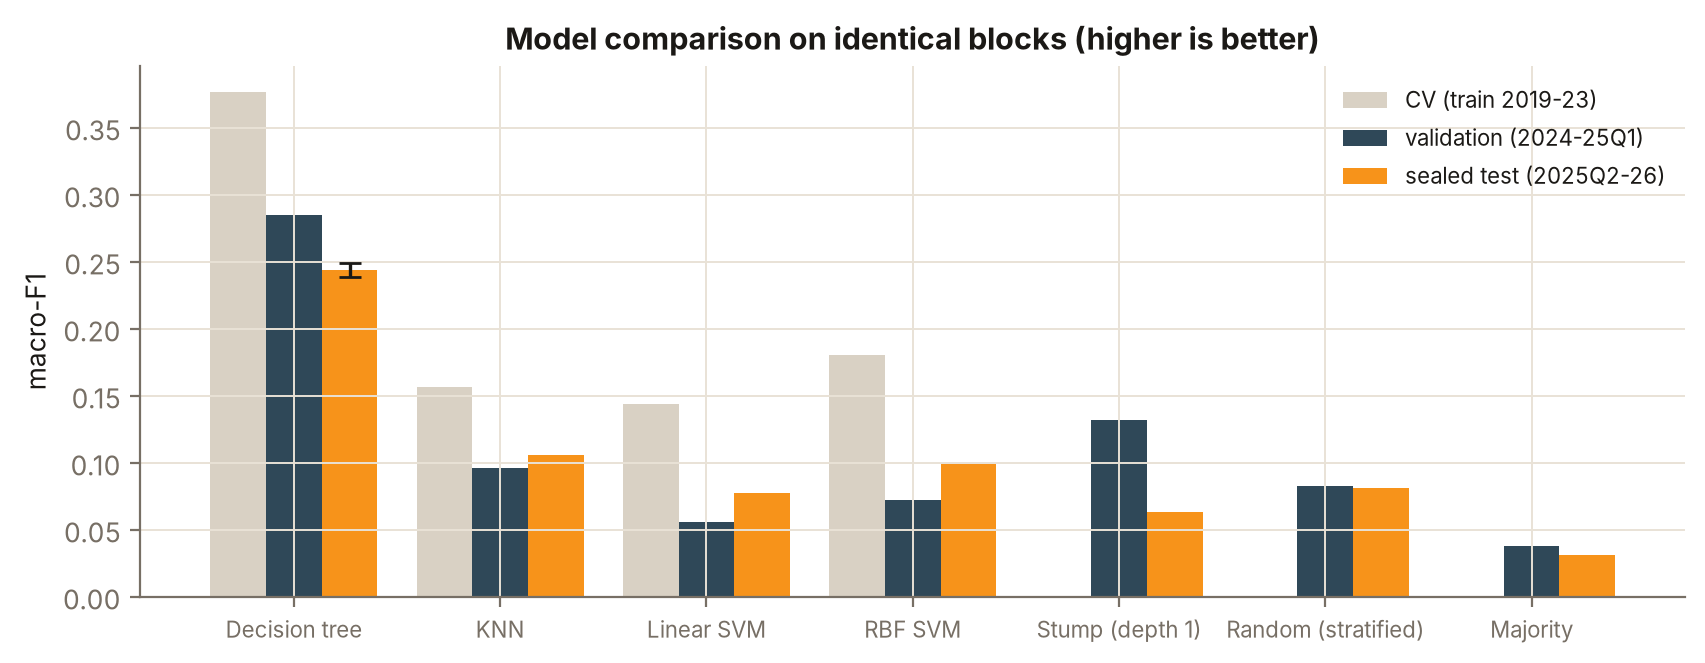
\includegraphics[keepaspectratio,alt={Macro-F1 of every model on CV, validation and the sealed test (same features, same blocks); error bar = day-block bootstrap 95\% interval.}]{figures/f07_model_comparison.png}}
\caption{Macro-F1 of every model on CV, validation and the sealed test
(same features, same blocks); error bar = day-block bootstrap 95\%
interval.}
\end{figure}

\textbf{Reading the numbers.} The decision tree is clearly the best
model: its macro-F1 is 3.0× the stratified-random baseline and 3.9× a
one-split tree. KNN and both SVMs also beat all three baselines, by
smaller margins. Exact-pool accuracy is modest (42\% across 12 classes,
against 18\% for always predicting the largest pool), but the
\textbf{true pool is among the tree's top three candidates 69\%} of the
time. In other words, behaviour narrows a block down to a few look-alike
pools; it cannot reliably separate pools that build blocks the same way.
Merging the template families fixed on training data raises accuracy
only to 46\%, because those families were defined from average profiles,
while the confusions below are spread across many large pools.

\textbf{Why the tree and not KNN or SVM?} The signal sits in a few
\emph{discrete} bit patterns (signal bits set, how many version bits are
rolled) and in thresholds on block composition. Axis-aligned tree splits
isolate exactly these patterns. Distance- and kernel-based models weigh
all 51 standardised features together, so a handful of informative bits
is drowned by many weakly informative ones (the curse of dimensionality
discussed in Lecture 7). We tested remedies on validation data --- only
the top-k mutual-information features, and mutual-information-weighted
distances --- and neither lifted KNN or the RBF SVM above about 0.11
macro-F1. The model comparison therefore teaches something about the
data: its geometry favours rule-like models.

\begin{figure}
\centering
\pandocbounded{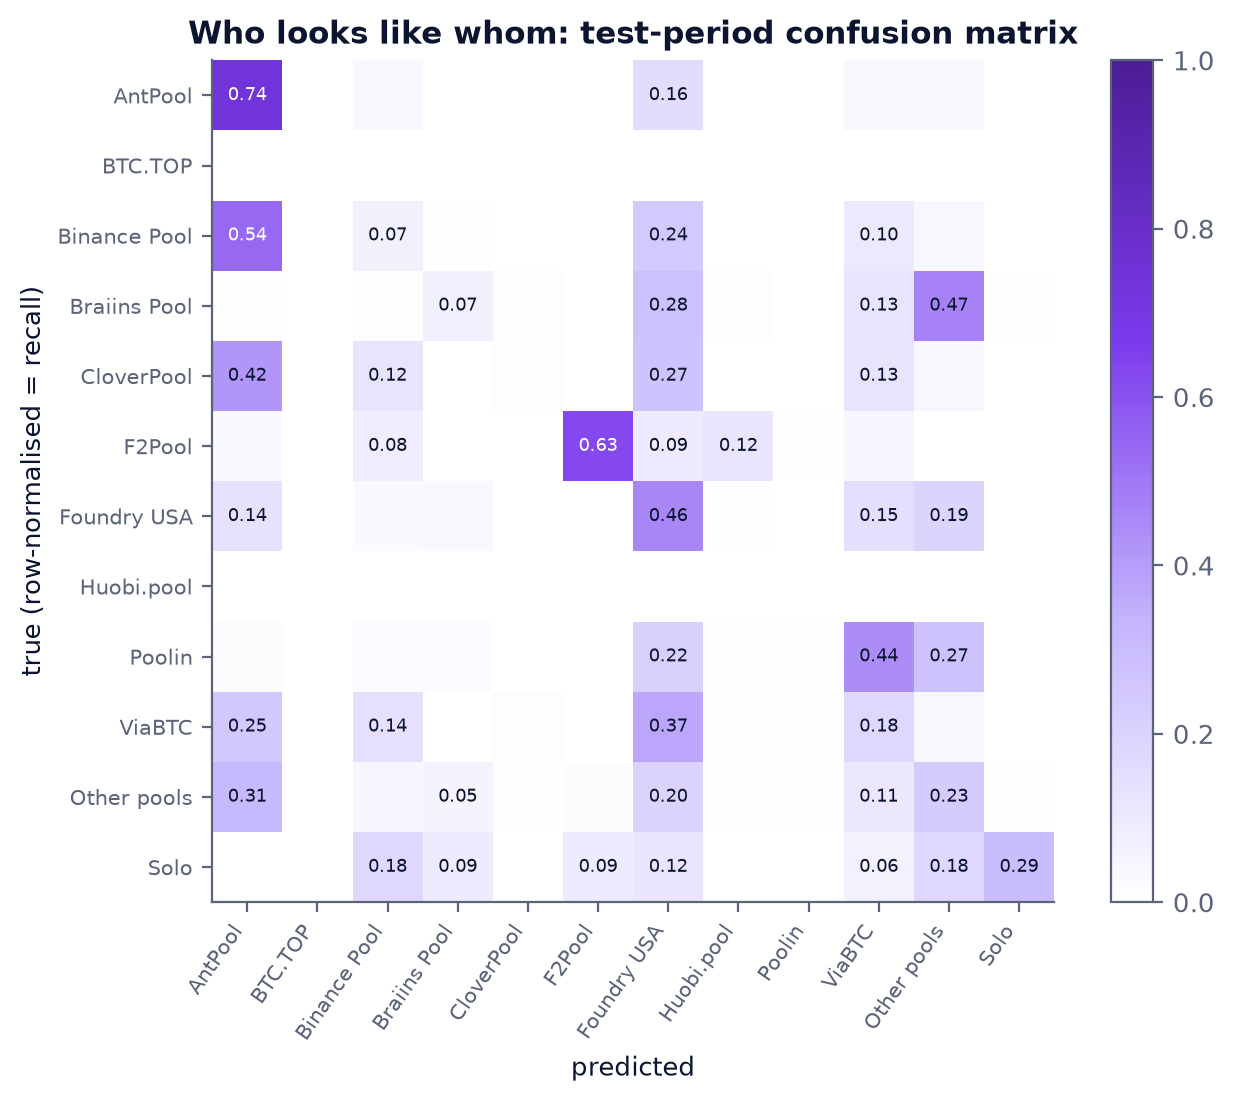
\includegraphics[keepaspectratio,alt={Test-period confusion matrix, row-normalised (diagonal = recall).}]{figures/f08_confusion.png}}
\caption{Test-period confusion matrix, row-normalised (diagonal =
recall).}
\end{figure}

\Needspace{23.8\baselineskip}\begin{reporttable}

\begin{longtable}[]{@{}lrrrr@{}}
\toprule\noalign{}
\textbf{Class} & \textbf{Precision} & \textbf{Recall} & \textbf{F1} &
\textbf{Blocks} \\
\midrule\noalign{}
\endhead
\bottomrule\noalign{}
\endlastfoot
AntPool & 0.45 & 0.74 & 0.56 & 15,241 \\
BTC.TOP & 0.00 & 0.00 & 0.00 & 0 \\
Binance Pool & 0.03 & 0.07 & 0.04 & 1,632 \\
Braiins Pool & 0.04 & 0.07 & 0.05 & 1,139 \\
CloverPool & 0.02 & 0.01 & 0.01 & 528 \\
F2Pool & 0.94 & 0.63 & 0.75 & 10,052 \\
Foundry USA & 0.48 & 0.46 & 0.47 & 23,960 \\
Huobi.pool & 0.00 & 0.00 & 0.00 & 0 \\
Poolin & 0.00 & 0.00 & 0.00 & 223 \\
ViaBTC & 0.18 & 0.18 & 0.18 & 8,944 \\
Other pools & 0.45 & 0.23 & 0.31 & 21,634 \\
Solo & 0.04 & 0.29 & 0.06 & 34 \\
\end{longtable}

\end{reporttable}

The validation-to-test difference and the monthly scores (dashboard,
Block Radar) show \textbf{drift}: pools change firmware and policies,
and new pools appear. The pools that did not exist (or were small)
during training are mapped by the frozen model as follows, a direct test
of ``whose template does a newcomer use?'':

\Needspace{17.4\baselineskip}\begin{reporttable}

\begin{longtable}[]{@{}lrlr@{}}
\toprule\noalign{}
\textbf{Newcomer pool} & \textbf{Blocks (val+test)} & \textbf{Most often
predicted as} & \textbf{Share} \\
\midrule\noalign{}
\endhead
\bottomrule\noalign{}
\endlastfoot
SpiderPool & 8,518 & Foundry USA & 29\% \\
MARA Pool & 6,940 & Other pools & 45\% \\
SECPOOL & 4,876 & AntPool & 67\% \\
Luxor & 4,443 & AntPool & 53\% \\
SBI Crypto & 2,262 & Other pools & 66\% \\
OCEAN & 1,666 & Solo & 18\% \\
WhitePool & 960 & Foundry USA & 49\% \\
Carbon Negative & 559 & Foundry USA & 50\% \\
\end{longtable}

\end{reporttable}

\subsection{The Solo class}\label{the-solo-class}

Solo blocks are a needle in a haystack (base rate 0.041\% of test
blocks). One-vs-rest \textbf{average precision} is the honest metric
here (ROC-AUC looks good for any rare class). The threshold frozen on
validation (highest recall with precision \textgreater= 0.5 on
validation) flagged 282 test blocks, of which 10 were solo (precision
4\%, recall 29\% of 34). With so few solo blocks per year these figures
carry wide uncertainty; the finding is that \textbf{modern solo blocks
are mostly built with the same open-source templates as pool blocks}
(section 10.3), so they are hard to fingerprint.

\begin{figure}
\centering
\pandocbounded{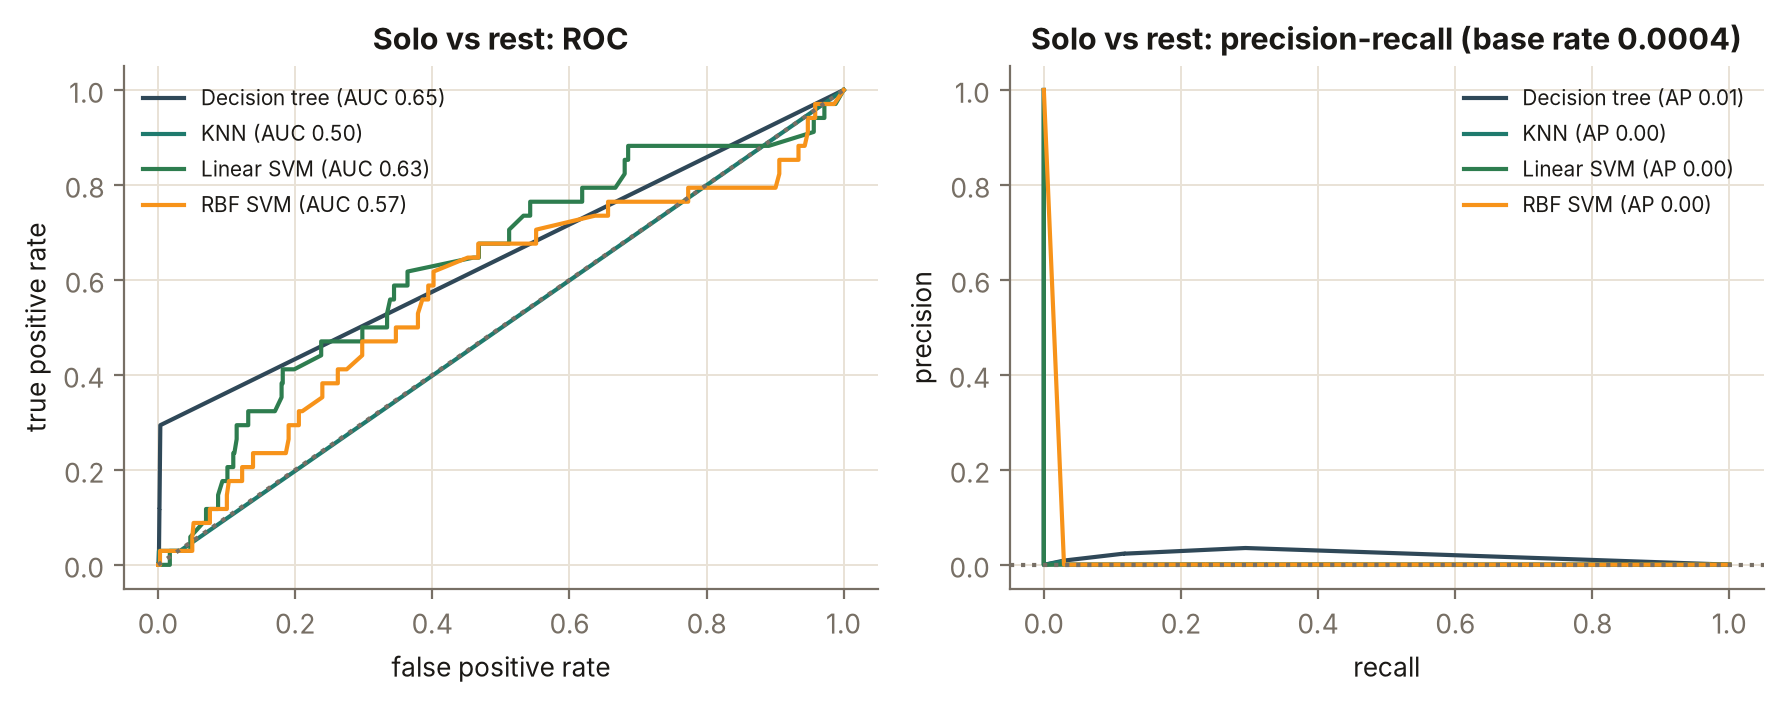
\includegraphics[keepaspectratio,alt={Solo vs rest on the test period: ROC (left) and precision-recall (right). SVM scores are decision values, not probabilities.}]{figures/f09_solo_roc_pr.png}}
\caption{Solo vs rest on the test period: ROC (left) and
precision-recall (right). SVM scores are decision values, not
probabilities.}
\end{figure}

\subsection{What the models rely on}\label{what-the-models-rely-on}

Permutation importance on the test period (drop in macro-F1 when one
feature is shuffled): \code{fullness} (0.1250),
\code{rel\_\allowbreak{}fullness} (0.0196),
\code{log\_\allowbreak{}min\_\allowbreak{}fee} (0.0109),
\code{fee\_\allowbreak{}share} (0.0088),
\code{log\_\allowbreak{}fee\_\allowbreak{}per\_\allowbreak{}kwu}
(0.0075), \code{witness\_\allowbreak{}tx\_\allowbreak{}share} (0.0061),
\code{ver\_\allowbreak{}roll\_\allowbreak{}popcount} (0.0041),
\code{witness\_\allowbreak{}byte\_\allowbreak{}share} (0.0019).
Version-rolling bits and how full a block is relative to that day
dominate; fee features matter less because, since 2023, most pools fill
blocks with the same fee-maximising template (section 10).

\textbf{KNN, opened up.} For the latest solo test block (\#973,413), the
41 nearest training blocks (euclidean distance, distance weights,
standardised features) voted AntPool: 9, Foundry USA: 8, Binance Pool:
8, ViaBTC: 6, so KNN predicted \textbf{AntPool}, a concrete illustration
of why solo blocks are hard: their nearest neighbours are ordinary pool
blocks.

\begin{figure}
\centering
\pandocbounded{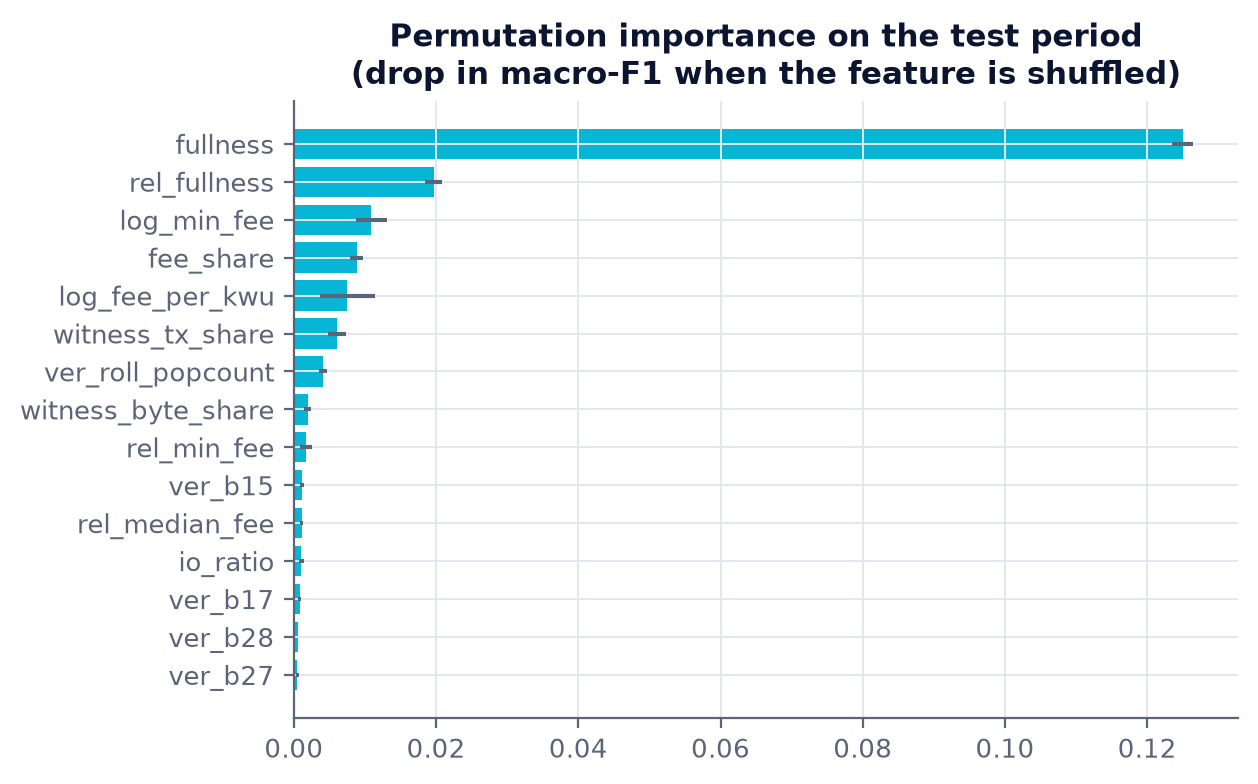
\includegraphics[keepaspectratio,alt={Permutation importance of the operational model on the test period.}]{figures/f10_permutation_importance.png}}
\caption{Permutation importance of the operational model on the test
period.}
\end{figure}

\section{Clustering}\label{clustering}

\subsection{Rediscovering the mining
eras}\label{rediscovering-the-mining-eras}

One row per week (926 weeks, 2009 → 2026), 9 standardised features
describing \emph{how} blocks were produced. K was chosen by the
silhouette maximum for K ≥ 3 (K = 2 trivially splits ``early'' from
``late''); 25 initialisations; a hand-checked first iteration confirms
the assignment and update steps (SSE 5,375.5 → 3,216.6, centroids
identical to scikit-learn within 2.8e-15). Stability across 10 seeds:
mean ARI 0.93.

\begin{figure}
\centering
\pandocbounded{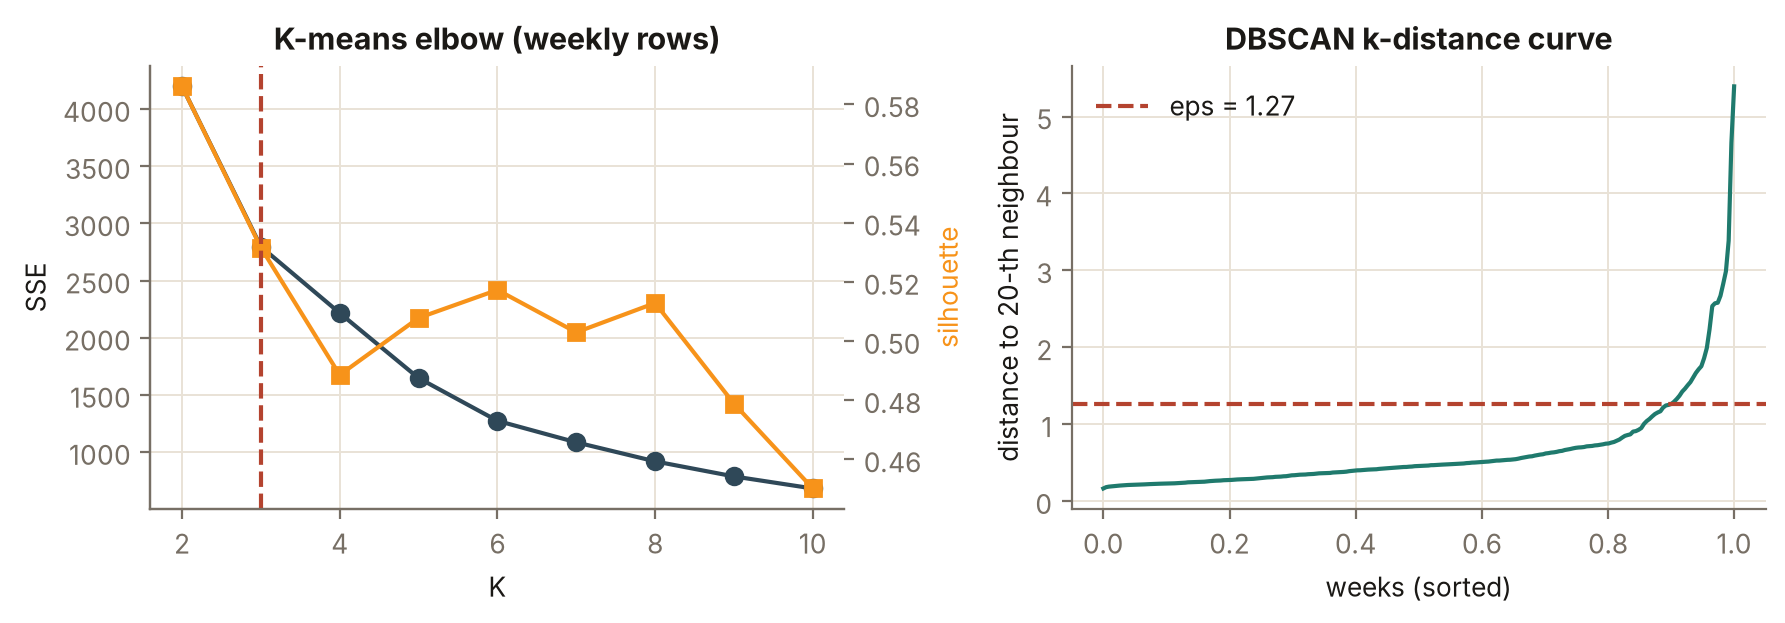
\includegraphics[keepaspectratio,alt={Left: K-means SSE (elbow) and silhouette by K. Right: DBSCAN k-distance curve with the chosen eps.}]{figures/f12_kmeans_dbscan.png}}
\caption{Left: K-means SSE (elbow) and silhouette by K. Right: DBSCAN
k-distance curve with the chosen eps.}
\end{figure}

\Needspace{9.4\baselineskip}\begin{reporttable}

\begin{longtable}[]{@{}
  >{\raggedright\arraybackslash}p{(\linewidth - 8\tabcolsep) * \real{0.1110}}
  >{\raggedleft\arraybackslash}p{(\linewidth - 8\tabcolsep) * \real{0.0850}}
  >{\raggedright\arraybackslash}p{(\linewidth - 8\tabcolsep) * \real{0.1500}}
  >{\raggedright\arraybackslash}p{(\linewidth - 8\tabcolsep) * \real{0.1500}}
  >{\raggedright\arraybackslash}p{(\linewidth - 8\tabcolsep) * \real{0.5040}}@{}}
\toprule\noalign{}
\begin{minipage}[b]{\linewidth}\raggedright
\textbf{Cluster}
\end{minipage} & \begin{minipage}[b]{\linewidth}\raggedleft
\textbf{Weeks}
\end{minipage} & \begin{minipage}[b]{\linewidth}\raggedright
\textbf{From}
\end{minipage} & \begin{minipage}[b]{\linewidth}\raggedright
\textbf{To}
\end{minipage} & \begin{minipage}[b]{\linewidth}\raggedright
\textbf{Dominant documented era}
\end{minipage} \\
\midrule\noalign{}
\endhead
\bottomrule\noalign{}
\endlastfoot
C0 & 123 & 2009-02-02 & 2011-06-06 & CPU \\
C1 & 179 & 2011-06-13 & 2014-12-29 & ASIC \\
C2 & 624 & 2014-11-10 & 2026-10-26 & Industrial ASIC \\
\end{longtable}

\end{reporttable}

\textbf{Without being told anything about hardware, the clusters line up
with the documented eras}: K-means ARI \textbf{0.71}, Ward linkage ARI
\textbf{0.89}. K-means places the start of the industrial regime in
2014-11, when pools had taken over and blocks had become full, rather
than at the first ASIC in January 2013; Ward linkage's boundaries fall
on 2011-06-13 and 2016-07-11, i.e.~two weeks after the documented start
of the FPGA era (1 June 2011) and two days after the July 2016 halving
that coincided with the industrial-ASIC (Antminer S9) era. Both are
useful refinements of a timeline that textbooks usually date by hardware
releases alone.

\Needspace{11.0\baselineskip}\begin{reporttable}

\begin{longtable}[]{@{}
  >{\raggedright\arraybackslash}p{(\linewidth - 8\tabcolsep) * \real{0.1240}}
  >{\raggedleft\arraybackslash}p{(\linewidth - 8\tabcolsep) * \real{0.2574}}
  >{\raggedright\arraybackslash}p{(\linewidth - 8\tabcolsep) * \real{0.3246}}
  >{\raggedleft\arraybackslash}p{(\linewidth - 8\tabcolsep) * \real{0.1590}}
  >{\raggedleft\arraybackslash}p{(\linewidth - 8\tabcolsep) * \real{0.1349}}@{}}
\toprule\noalign{}
\begin{minipage}[b]{\linewidth}\raggedright
\textbf{Linkage}
\end{minipage} & \begin{minipage}[b]{\linewidth}\raggedleft
\textbf{Cophenetic correlation}
\end{minipage} & \begin{minipage}[b]{\linewidth}\raggedright
\textbf{Cluster sizes (cut at K)}
\end{minipage} & \begin{minipage}[b]{\linewidth}\raggedleft
\textbf{ARI vs K-means}
\end{minipage} & \begin{minipage}[b]{\linewidth}\raggedleft
\textbf{ARI vs eras}
\end{minipage} \\
\midrule\noalign{}
\endhead
\bottomrule\noalign{}
\endlastfoot
single & 0.882 & 921, 4, 1 & 0.02 & 0.01 \\
complete & 0.904 & 818, 103, 5 & 0.41 & 0.29 \\
average & 0.930 & 900, 21, 5 & 0.08 & 0.06 \\
ward & 0.808 & 538, 265, 123 & 0.71 & 0.89 \\
\end{longtable}

\end{reporttable}

Single linkage chains almost everything into one cluster (its known
weakness); average linkage preserves distances best (highest cophenetic
correlation) but also produces one dominant cluster; \textbf{Ward},
which minimises the increase in SSE, gives compact eras closest to
history. \textbf{DBSCAN} (MinPts 20, eps 1.27 from the 0.9 quantile of
the k-distance curve) finds 2 dense regions and labels 4.5\% of weeks as
noise: the transition weeks where hash rate and block composition were
changing fastest. Density-based clustering is the wrong tool for
separating eras that blend into each other, and that is itself a
finding.

\begin{figure}
\centering
\pandocbounded{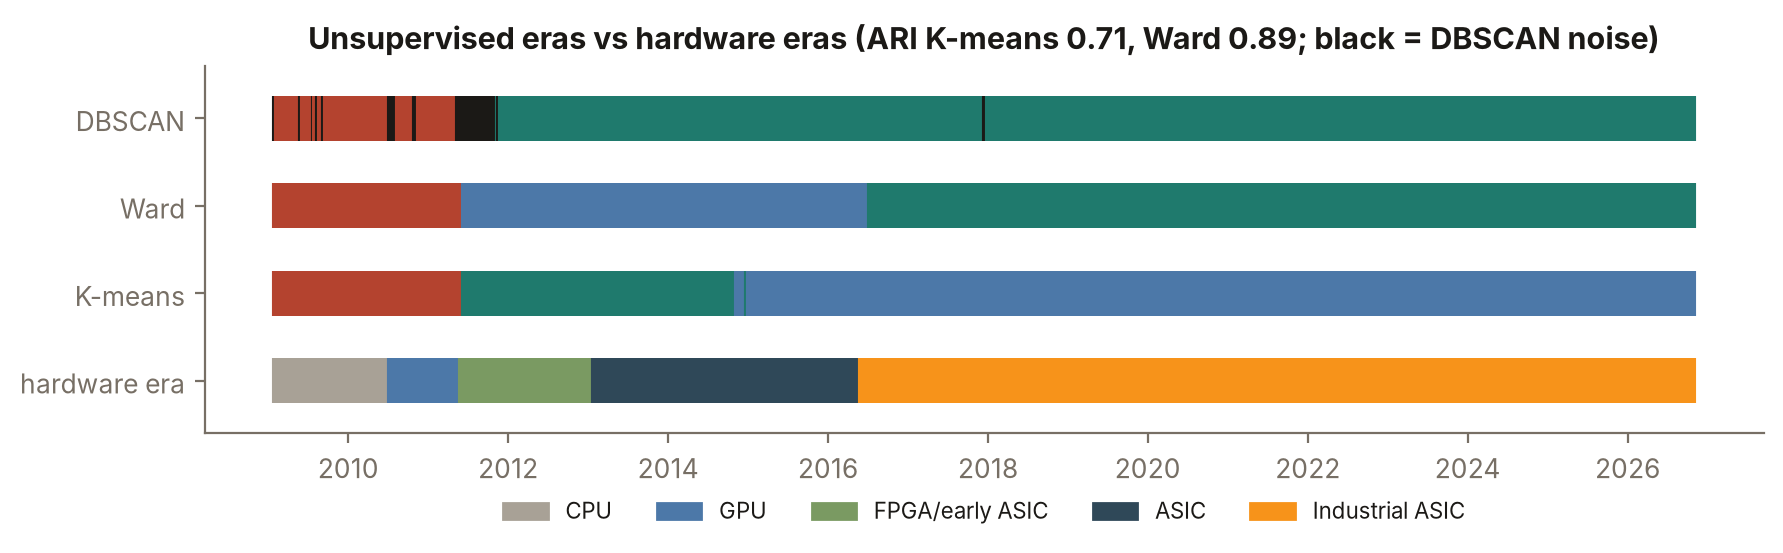
\includegraphics[keepaspectratio,alt={Weekly cluster assignments compared with the documented hardware eras (black = DBSCAN noise).}]{figures/f13_eras_timeline.png}}
\caption{Weekly cluster assignments compared with the documented
hardware eras (black = DBSCAN noise).}
\end{figure}

\subsection{Pool families}\label{pool-families}

For the 19 pools with at least 300 blocks in 2024-01-01 → 2026-11-01, a
profile of mean fingerprints (version-rolling habits, signal bits,
empty-block rate, day-relative fee and size policy, timestamp offset)
was clustered with average linkage (cophenetic correlation 0.858).
Cutting below the 35th percentile of merge heights gives these
multi-pool families: \textbf{AntPool + Braiins Pool + Foundry USA +
Luxor}; \textbf{Binance Pool + CloverPool + Poolin}; \textbf{SECPOOL +
ULTIMUSPOOL}.

\begin{figure}
\centering
\pandocbounded{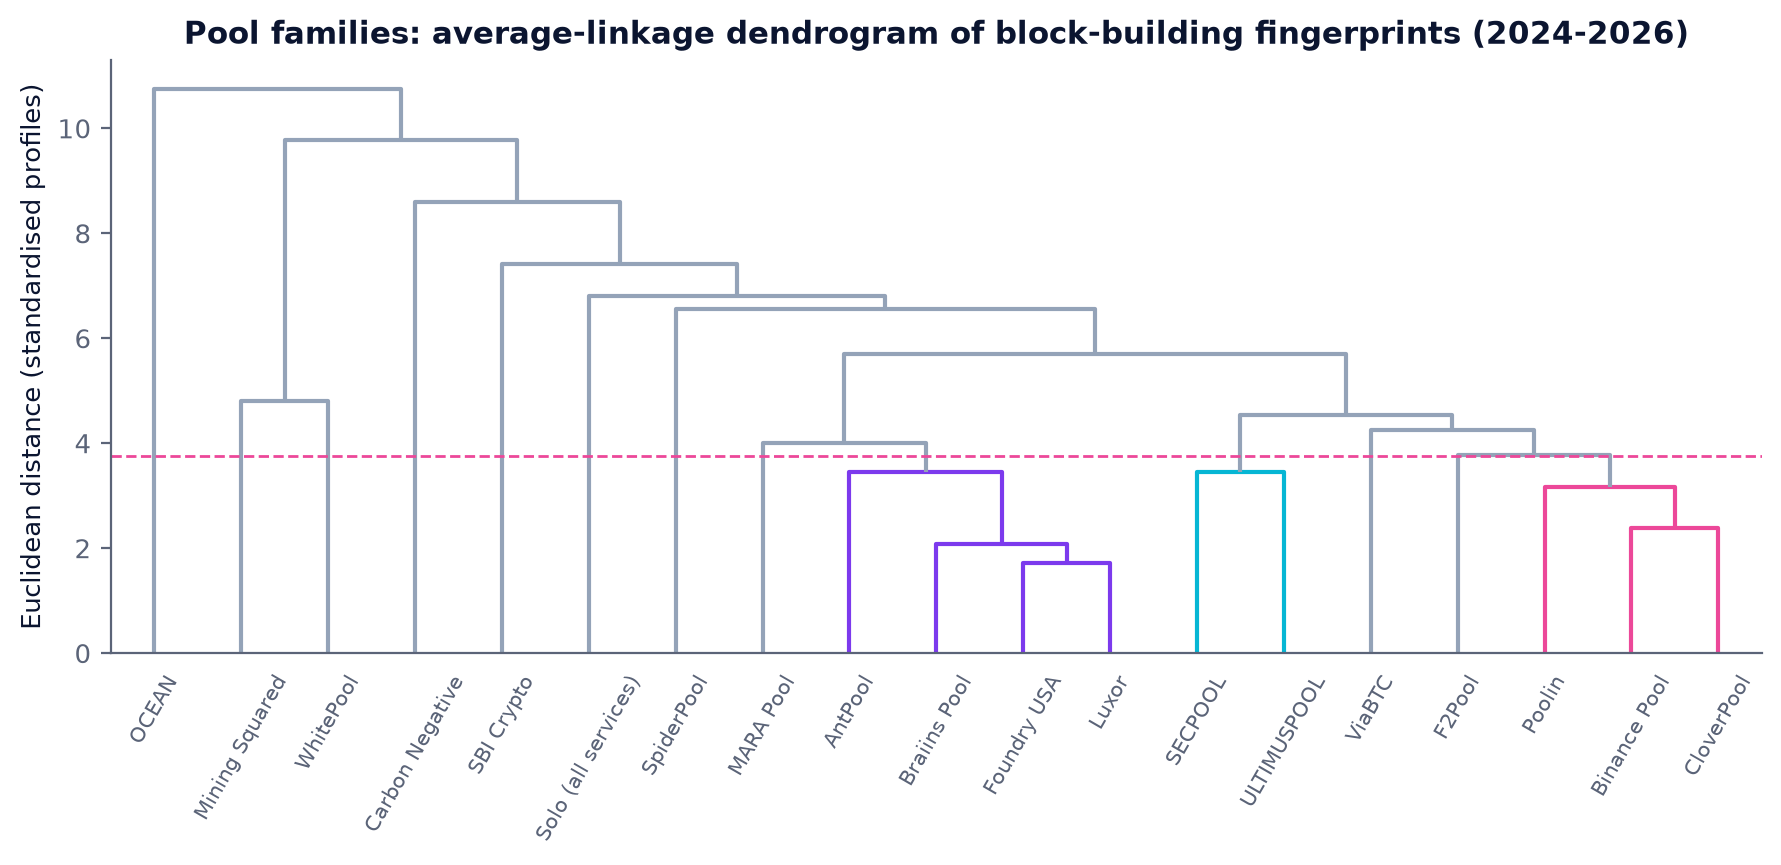
\includegraphics[keepaspectratio,alt={Average-linkage dendrogram of pool fingerprint profiles (2024-2026); the dashed line is the family cut.}]{figures/f14_pool_dendrogram.png}}
\caption{Average-linkage dendrogram of pool fingerprint profiles
(2024-2026); the dashed line is the family cut.}
\end{figure}

The families largely agree with the classifier: pools that are rare or
absent in training are mostly read as an existing pool with a similar
fingerprint (SECPOOL → AntPool 67\%; Luxor → AntPool 53\%; SBI Crypto →
Other pools 66\%; WhitePool → Foundry USA 49\%), and Luxor is read as
AntPool, which the dendrogram places in the same family. This matters
for decentralisation: block production that looks spread over many pool
names may come from fewer distinct block-building set-ups. Similar
fingerprints can also come from shared mining firmware or pool software,
so the data \textbf{suggest}, but do not prove, common control.

\subsection{Anomalous blocks}\label{anomalous-blocks}

DBSCAN on 6,000 recent blocks marks 1.5\% as noise. Those blocks are 65×
more often empty than average and have unusual timestamps, which is
genuine but rare miner behaviour, not data errors.

\section{Association rules}\label{association-rules}

\subsection{Transactions, items and
Apriori}\label{transactions-items-and-apriori}

Each modern block (2023-01-01 → 2025-04-01, \textbf{120,538
transactions}) is a basket of 33 items: empty, full (≥ 98\%) or light;
how many version bits are rolled (none, 1-4, 5-8, 9-12, 13-16); signal
bits set; timestamp far ahead of the median; fast or slow follow-up;
fees and transaction count below or above the day's median;
witness-heavy content; consolidating or fan-out shape; and the miner
(pools with at least 1\% of blocks, ``small pools'', Solo, Unknown). Bin
edges were fitted on the discovery window only.

Apriori was implemented from scratch: join frequent (k−1)-itemsets
sharing k−2 items, prune every candidate with an infrequent subset
(support is anti-monotone), then count the survivors.

\Needspace{11.0\baselineskip}\begin{reporttable}

\begin{longtable}[]{@{}rrrrr@{}}
\toprule\noalign{}
\textbf{k} & \textbf{Joined candidates} & \textbf{Pruned by subset} &
\textbf{Counted} & \textbf{Frequent} \\
\midrule\noalign{}
\endhead
\bottomrule\noalign{}
\endlastfoot
1 & 33 & 0 & 33 & 30 \\
2 & 435 & 0 & 435 & 170 \\
3 & 1,082 & 531 & 551 & 345 \\
4 & 1,158 & 765 & 393 & 292 \\
\end{longtable}

\end{reporttable}

Minimum support 1\% (1,206 blocks) gave 837 frequent itemsets. An
exhaustive brute-force count of every itemset up to size 3 over 12 items
found the same 40 frequent itemsets with identical counts (\textbf{check
passed}).

\subsection{Rules ``block properties →
miner''}\label{rules-block-properties-miner}

With minimum confidence 30\% (single pools have base rates of 1-30\%, so
this already implies lift \textgreater{} 1), 103 rules were found, and
each was re-measured on the later window 2025-04-01 → 2026-11-01.

\Needspace{17.4\baselineskip}\begin{reporttablesmall}

\begin{longtable}[]{@{}
  >{\raggedright\arraybackslash}p{(\linewidth - 10\tabcolsep) * \real{0.4570}}
  >{\raggedleft\arraybackslash}p{(\linewidth - 10\tabcolsep) * \real{0.0941}}
  >{\raggedleft\arraybackslash}p{(\linewidth - 10\tabcolsep) * \real{0.1271}}
  >{\raggedleft\arraybackslash}p{(\linewidth - 10\tabcolsep) * \real{0.0720}}
  >{\raggedleft\arraybackslash}p{(\linewidth - 10\tabcolsep) * \real{0.1337}}
  >{\raggedright\arraybackslash}p{(\linewidth - 10\tabcolsep) * \real{0.1161}}@{}}
\toprule\noalign{}
\begin{minipage}[b]{\linewidth}\raggedright
\textbf{Rule}
\end{minipage} & \begin{minipage}[b]{\linewidth}\raggedleft
\textbf{Support}
\end{minipage} & \begin{minipage}[b]{\linewidth}\raggedleft
\textbf{Confidence}
\end{minipage} & \begin{minipage}[b]{\linewidth}\raggedleft
\textbf{Lift}
\end{minipage} & \begin{minipage}[b]{\linewidth}\raggedleft
\textbf{Later confidence}
\end{minipage} & \begin{minipage}[b]{\linewidth}\raggedright
\textbf{Confirmed}
\end{minipage} \\
\midrule\noalign{}
\endhead
\bottomrule\noalign{}
\endlastfoot
fullness=full(\textgreater=98\%) ∧ version=signal bits set → SBI Crypto
& 1.5\% & 65\% & 42.97 & 80\% & yes \\
version=signal bits set → SBI Crypto & 1.5\% & 61\% & 40.63 & 85\% &
yes \\
fullness=full(\textgreater=98\%) ∧ version=rolls 5-8 bits ∧
interval=fast(\textless60s) → Foundry USA & 1.3\% & 39\% & 1.29 & 36\% &
yes \\
version=rolls 5-8 bits ∧ interval=fast(\textless60s) → Foundry USA &
1.3\% & 38\% & 1.26 & 32\% & no \\
version=rolls 5-8 bits ∧ interval=fast(\textless60s) ∧
fees=below-day-median → Foundry USA & 1.2\% & 38\% & 1.25 & 34\% & no \\
version=rolls 5-8 bits ∧ txcount=below-day-median ∧
content=witness-heavy → Foundry USA & 1.9\% & 37\% & 1.23 & 34\% & no \\
version=rolls 5-8 bits ∧ content=witness-heavy ∧ shape=consolidating →
Foundry USA & 1.4\% & 37\% & 1.23 & 34\% & yes \\
version=rolls 9-12 bits ∧ txcount=below-day-median ∧ shape=consolidating
→ Foundry USA & 1.1\% & 37\% & 1.22 & 31\% & no \\
\end{longtable}

\end{reporttablesmall}

Confidence is a historical conditional frequency and lift compares it
with the miner's base rate; neither implies causation. Most
high-confidence rules point to the largest pool simply because of its
base rate (low lift); the informative rules are the high-lift ones.

\begin{figure}
\centering
\pandocbounded{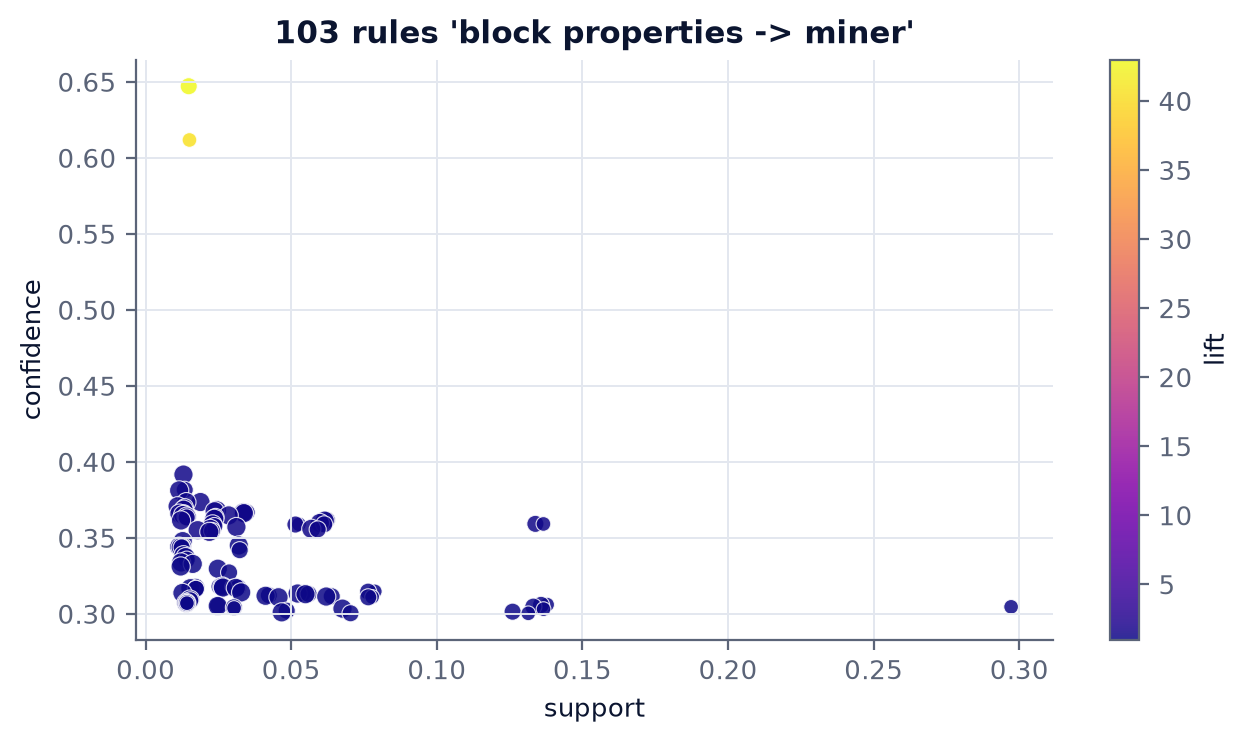
\includegraphics[keepaspectratio,alt={Rules by support and confidence, coloured by lift.}]{figures/f15_rules.png}}
\caption{Rules by support and confidence, coloured by lift.}
\end{figure}

\subsection{Pool signatures and the solo
contrast}\label{pool-signatures-and-the-solo-contrast}

Small pools can never pass a global support threshold, so we also mined
frequent itemsets \textbf{inside} each pool's blocks and compared their
support with all other blocks (contrast mining):

\Needspace{17.4\baselineskip}\begin{reporttable}

\begin{longtable}[]{@{}
  >{\raggedright\arraybackslash}p{(\linewidth - 8\tabcolsep) * \real{0.1500}}
  >{\raggedright\arraybackslash}p{(\linewidth - 8\tabcolsep) * \real{0.5300}}
  >{\raggedleft\arraybackslash}p{(\linewidth - 8\tabcolsep) * \real{0.0720}}
  >{\raggedleft\arraybackslash}p{(\linewidth - 8\tabcolsep) * \real{0.1370}}
  >{\raggedleft\arraybackslash}p{(\linewidth - 8\tabcolsep) * \real{0.1110}}@{}}
\toprule\noalign{}
\begin{minipage}[b]{\linewidth}\raggedright
\textbf{Pool}
\end{minipage} & \begin{minipage}[b]{\linewidth}\raggedright
\textbf{Signature itemset}
\end{minipage} & \begin{minipage}[b]{\linewidth}\raggedleft
\textbf{In pool}
\end{minipage} & \begin{minipage}[b]{\linewidth}\raggedleft
\textbf{Elsewhere}
\end{minipage} & \begin{minipage}[b]{\linewidth}\raggedleft
\textbf{Ratio}
\end{minipage} \\
\midrule\noalign{}
\endhead
\bottomrule\noalign{}
\endlastfoot
SBI Crypto & fullness=full(\textgreater=98\%) ∧ version=rolls 1-4 bits ∧
version=signal bits set & 51\% & 0.3\% & 175.4× \\
Braiins Pool & fullness=full(\textgreater=98\%) ∧ version=signal bits
set & 39\% & 1.7\% & 23.6× \\
MARA Pool & fullness=full(\textgreater=98\%) ∧ version=rolls 5-8 bits &
62\% & 36.3\% & 1.7× \\
ViaBTC & fullness=full(\textgreater=98\%) ∧ version=rolls 1-4 bits &
49\% & 33.4\% & 1.5× \\
Binance Pool & version=rolls 1-4 bits & 48\% & 35.5\% & 1.3× \\
CloverPool & version=rolls 1-4 bits & 47\% & 36.0\% & 1.3× \\
Foundry USA & fullness=full(\textgreater=98\%) ∧ version=rolls 5-8 bits
& 44\% & 34.3\% & 1.3× \\
SECPOOL & fullness=full(\textgreater=98\%) ∧ version=rolls 1-4 bits &
45\% & 35.1\% & 1.3× \\
\end{longtable}

\end{reporttable}

Pools with a strong signature (signal bits, distinctive version rolling)
are exactly the ones the classifier recognises best. The large pools
(AntPool, F2Pool, Luxor, SpiderPool) have \textbf{no distinctive itemset
at all}: they build blocks the way everybody else does. For the 85 solo
blocks since 2019, the most over-represented itemset
(txcount=below-day-median ∧ shape=consolidating) is only 1.24× more
common than among pool blocks, confirming that modern solo blocks are
nearly indistinguishable from pool blocks.

\section{Decision making on new
examples}\label{decision-making-on-new-examples}

\subsection{Unattributed blocks and real
concentration}\label{unattributed-blocks-and-real-concentration}

In the last 12 months before the freeze, 92 of 52,360 blocks (0.18\%)
carried no attribution. The frozen model attributes them as Other pools:
68, Braiins Pool: 13, ViaBTC: 4, Foundry USA: 3. By pool \emph{name},
\textbf{3 entities} mined more than half of the blocks (the Nakamoto
coefficient). As an \textbf{upper-bound scenario}, if every fingerprint
family of section 9.2 were a single block builder, the number would be
\textbf{1} (largest family: AntPool + Braiins Pool + Foundry USA +
Luxor). Similarity is not proof of shared ownership (family merges come
from fingerprint similarity (section 9), which suggests but does not
prove common control; shared templates can also come from shared
software or proxy arrangements), so the true figure lies between these
two bounds; the point is that pool names alone cannot establish how
decentralised block building is.

\begin{figure}
\centering
\pandocbounded{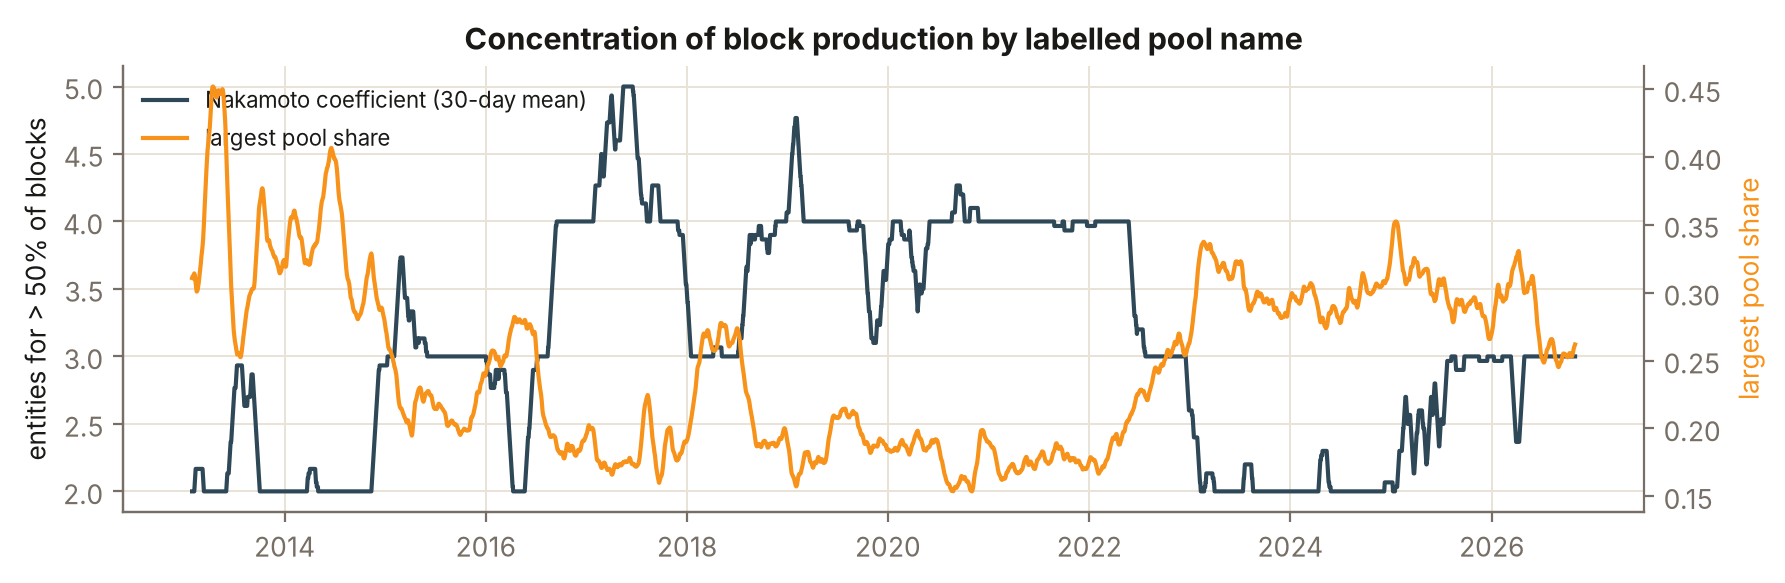
\includegraphics[keepaspectratio,alt={Concentration of block production by labelled pool name.}]{figures/f18_concentration.png}}
\caption{Concentration of block production by labelled pool name.}
\end{figure}

\subsection{Blocks mined after the data
freeze}\label{blocks-mined-after-the-data-freeze}

The 1,446 labelled blocks mined between 2026-11-01 and 2026-11-12 were
never seen by any stage. The frozen model predicted their miner first;
when the labels were revealed, \textbf{36.1\%} were correct, below the
test-period accuracy (42\%): one more sign of drift, as pools such as
SpiderPool keep growing after the training period. The command
\code{uv run hashatlas predict --heights …} repeats this for any block.

\subsection{The miner advisor: pool, solo lottery, or switch
off?}\label{the-miner-advisor-pool-solo-lottery-or-switch-off}

At the freeze (30-day means to 2026-10-31): network hash rate 1,032
EH/s, BTC price 82,285 USD, \textbf{hash price 0.0380 USD per TH/s per
day}. For a device with hash rate h (TH/s) and power W, pool income =
hash price × h × (1 − 2\% fee), electricity = W/1000 × 24 × price per
kWh, and solo blocks arrive as a Poisson process with rate (h / network)
× 144 per day.

\Needspace{11.0\baselineskip}\begin{reporttable}

\begin{longtable}[]{@{}
  >{\raggedright\arraybackslash}p{(\linewidth - 10\tabcolsep) * \real{0.2142}}
  >{\raggedleft\arraybackslash}p{(\linewidth - 10\tabcolsep) * \real{0.1701}}
  >{\raggedleft\arraybackslash}p{(\linewidth - 10\tabcolsep) * \real{0.1892}}
  >{\raggedleft\arraybackslash}p{(\linewidth - 10\tabcolsep) * \real{0.1136}}
  >{\raggedleft\arraybackslash}p{(\linewidth - 10\tabcolsep) * \real{0.1712}}
  >{\raggedleft\arraybackslash}p{(\linewidth - 10\tabcolsep) * \real{0.1418}}@{}}
\toprule\noalign{}
\begin{minipage}[b]{\linewidth}\raggedright
\textbf{Device}
\end{minipage} & \begin{minipage}[b]{\linewidth}\raggedleft
\textbf{HK pool income / day}
\end{minipage} & \begin{minipage}[b]{\linewidth}\raggedleft
\textbf{HK electricity / day}
\end{minipage} & \begin{minipage}[b]{\linewidth}\raggedleft
\textbf{Profit / day}
\end{minipage} & \begin{minipage}[b]{\linewidth}\raggedleft
\textbf{Break-even USD/kWh}
\end{minipage} & \begin{minipage}[b]{\linewidth}\raggedleft
\textbf{Solo odds / year}
\end{minipage} \\
\midrule\noalign{}
\endhead
\bottomrule\noalign{}
\endlastfoot
Bitaxe-class home miner & 0.04 & 0.08 & -0.03 & 0.103 & 1 in 16,362 \\
Antminer S19j Pro & 3.87 & 12.89 & -9.02 & 0.053 & 1 in 189 \\
Antminer S21 & 7.44 & 14.70 & -7.26 & 0.089 & 1 in 99 \\
Antminer S21 XP Hyd & 17.59 & 23.84 & -6.25 & 0.129 & 1 in 42 \\
\end{longtable}

\end{reporttable}

Hong Kong business electricity costs 0.175 USD/kWh; an Antminer S21
needs \textbf{0.089 USD/kWh or less}. Among the 26 economies with
business tariffs in our snapshot, the S21 covers its electricity in 6:
Bhutan, Ethiopia, Paraguay, Indonesia, Vietnam, Kazakhstan.

\begin{figure}
\centering
\pandocbounded{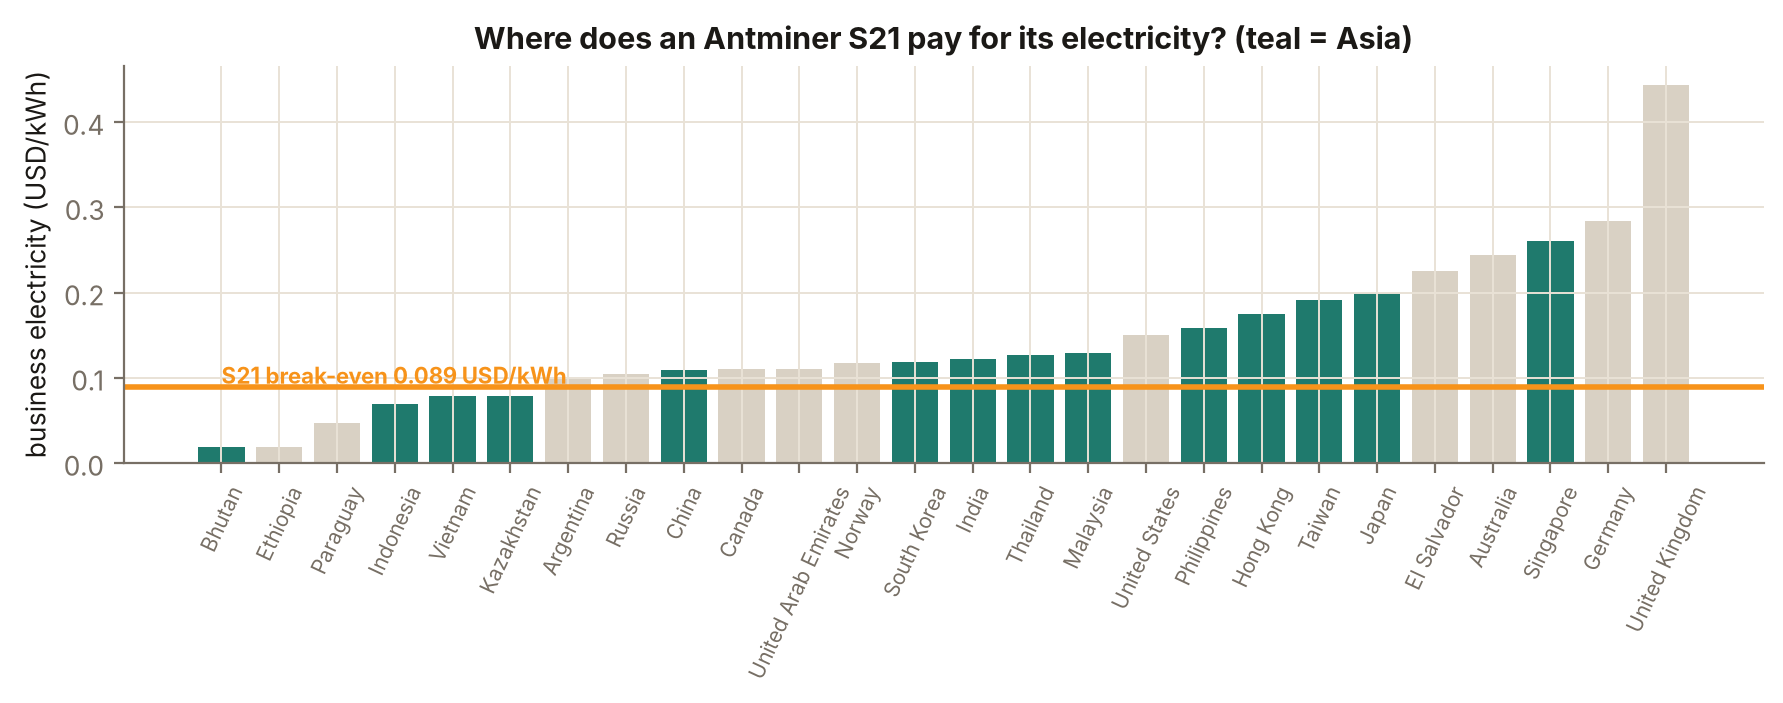
\includegraphics[keepaspectratio,alt={Business electricity price by economy against the Antminer S21 break-even price (teal = Asia).}]{figures/f16_advisor.png}}
\caption{Business electricity price by economy against the Antminer S21
break-even price (teal = Asia).}
\end{figure}

\textbf{Decision.} In Hong Kong, at retail tariffs, mining for profit
does not pay at the freeze-date hash price. A small home miner (1.2
TH/s) is a lottery ticket: odds of about \textbf{1 in 16,362 per year},
an expected wait of 16,361 years, and it costs electricity every day it
runs. The advisor recommends pool mining only where electricity is below
the device's break-even price, and labels solo mining honestly as a
lottery.

\begin{figure}
\centering
\pandocbounded{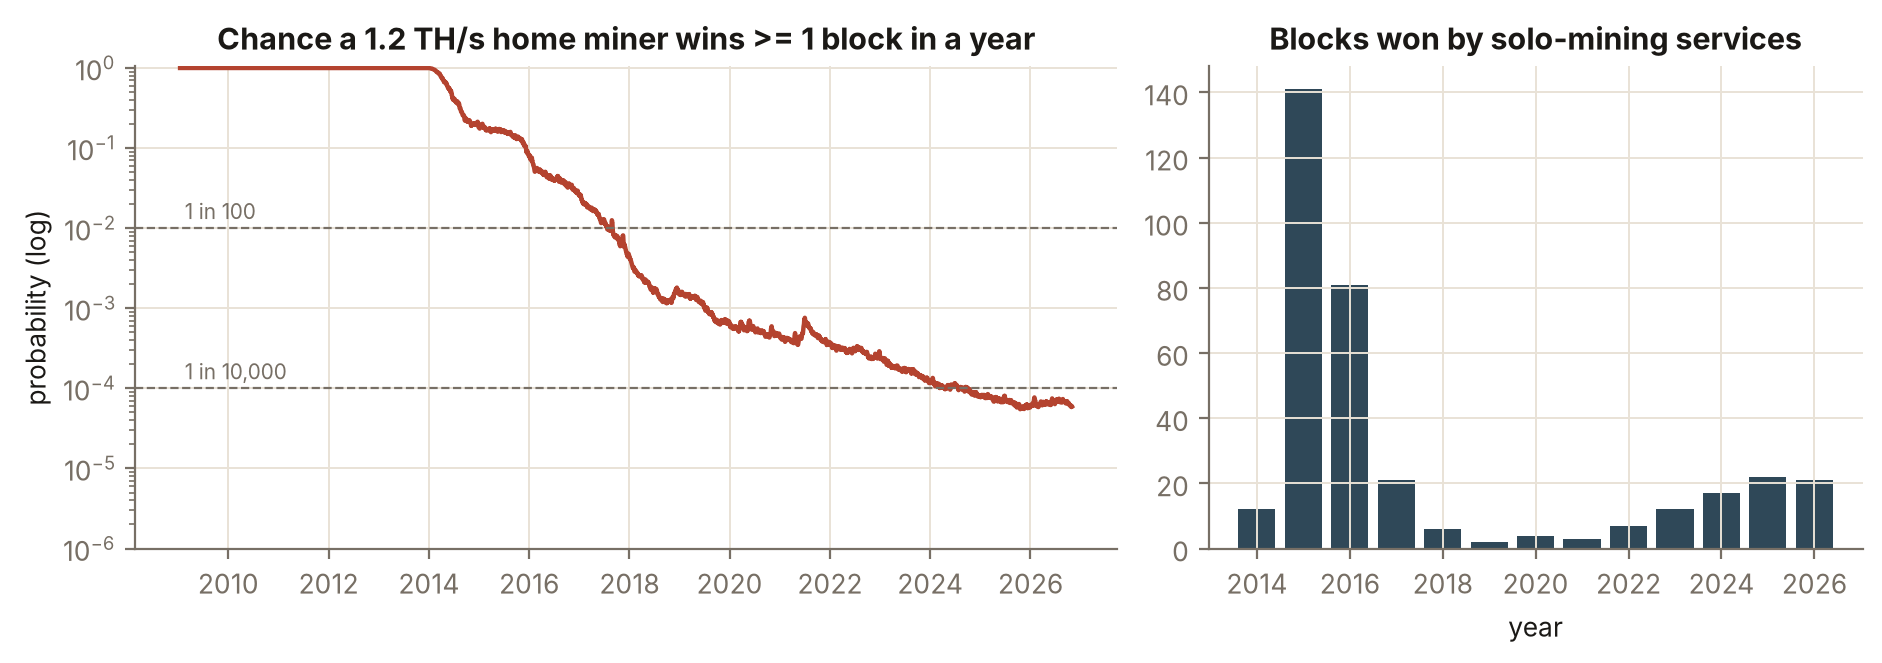
\includegraphics[keepaspectratio,alt={Chance that a 1.2 TH/s miner finds at least one block in a year (left) and blocks actually won by solo services (right).}]{figures/f03_solo_odds.png}}
\caption{Chance that a 1.2 TH/s miner finds at least one block in a year
(left) and blocks actually won by solo services (right).}
\end{figure}

\section{Future Lab: the 2028 halving (scenarios, not
forecasts)}\label{future-lab-the-2028-halving-scenarios-not-forecasts}

\textbf{How much future, and how.} We include the future only where it
can be grounded: (1) the protocol schedule is certain: the subsidy
halves at height 1,050,000; (2) hash-rate growth is simulated by
block-bootstrapping 30-day stretches of historical daily growth (4,000
paths); (3) BTC price and fee share are \textbf{user-chosen scenarios},
never forecasts; (4) the method is \textbf{backtested} from four
historical dates.

\begin{itemize}
\tightlist
\item
  Projected halving date: \textbf{2028-04-07} (80\% of paths 2028-04-04
  → 2028-04-09).
\item
  Backtest (16 origin/horizon cases): the 80\% band contained the
  realised hash rate in \textbf{75\%} of cases. Two resampling windows
  were compared by the declared rule ``lower backtest error wins'': mean
  \textbar error\textbar{} of the median path 50\% (last 3 years) vs
  72\% (since 2017), so the last-3-years window drives the main
  scenario. \textbf{Honest limitation:} a naive ``no growth'' projection
  had a lower error (28\%) over 2019-2025, so the median path should be
  read as one point in a wide range, not as a prediction.
\end{itemize}

\begin{figure}
\centering
\pandocbounded{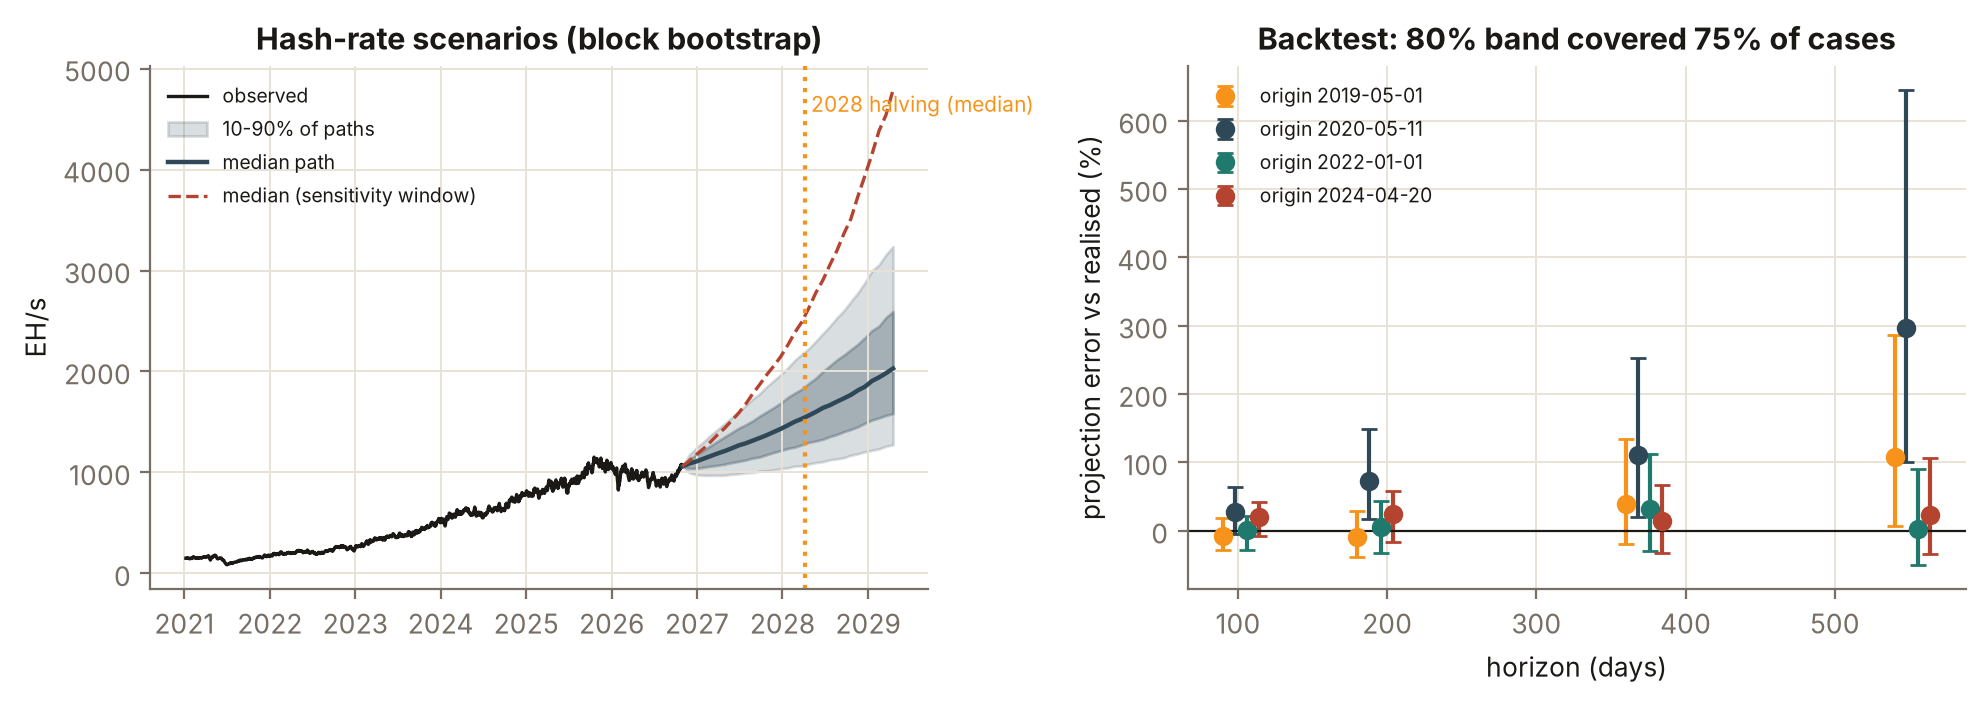
\includegraphics[keepaspectratio,alt={Left: hash-rate scenarios to 2029 with the projected 2028 halving. Right: backtest error of the same method from past origins.}]{figures/f17_future.png}}
\caption{Left: hash-rate scenarios to 2029 with the projected 2028
halving. Right: backtest error of the same method from past origins.}
\end{figure}

\Needspace{19.0\baselineskip}\begin{reporttable}

\begin{longtable}[]{@{}
  >{\raggedright\arraybackslash}p{(\linewidth - 8\tabcolsep) * \real{0.2206}}
  >{\raggedright\arraybackslash}p{(\linewidth - 8\tabcolsep) * \real{0.2161}}
  >{\raggedright\arraybackslash}p{(\linewidth - 8\tabcolsep) * \real{0.1500}}
  >{\raggedleft\arraybackslash}p{(\linewidth - 8\tabcolsep) * \real{0.2641}}
  >{\raggedleft\arraybackslash}p{(\linewidth - 8\tabcolsep) * \real{0.1492}}@{}}
\toprule\noalign{}
\begin{minipage}[b]{\linewidth}\raggedright
\textbf{Device}
\end{minipage} & \begin{minipage}[b]{\linewidth}\raggedright
\textbf{Checkpoint}
\end{minipage} & \begin{minipage}[b]{\linewidth}\raggedright
\textbf{Date}
\end{minipage} & \begin{minipage}[b]{\linewidth}\raggedleft
\textbf{Break-even USD/kWh (p10-p90)}
\end{minipage} & \begin{minipage}[b]{\linewidth}\raggedleft
\textbf{Solo odds / year}
\end{minipage} \\
\midrule\noalign{}
\endhead
\bottomrule\noalign{}
\endlastfoot
Bitaxe-class home miner & 2027-01-01 & 2027-01-01 & 0.096 (0.086-0.108)
& 1 in 17,607 \\
Bitaxe-class home miner & one month after halving & 2028-05-07 & 0.034
(0.023-0.049) & 1 in 25,114 \\
Bitaxe-class home miner & 2029-01-01 & 2029-01-01 & 0.029 (0.018-0.044)
& 1 in 29,793 \\
Antminer S21 & 2027-01-01 & 2027-01-01 & 0.082 (0.074-0.093) & 1 in
106 \\
Antminer S21 & one month after halving & 2028-05-07 & 0.029
(0.020-0.042) & 1 in 151 \\
Antminer S21 & 2029-01-01 & 2029-01-01 & 0.024 (0.016-0.038) & 1 in
179 \\
Antminer S21 XP Hyd & 2027-01-01 & 2027-01-01 & 0.120 (0.107-0.136) & 1
in 45 \\
Antminer S21 XP Hyd & one month after halving & 2028-05-07 & 0.042
(0.029-0.061) & 1 in 64 \\
Antminer S21 XP Hyd & 2029-01-01 & 2029-01-01 & 0.036 (0.023-0.055) & 1
in 76 \\
\end{longtable}

\end{reporttable}

At today's price and a 5\% fee share, the halving cuts the break-even
electricity price of every device by more than half (Antminer S21: 0.082
→ 0.029 USD/kWh). Break-even scales linearly with price, so even a
doubled BTC price would only restore it to about 0.058 USD/kWh. After
2028, mining is viable only at very cheap, mostly industrial or stranded
power, consistent with how mining migrated after earlier halvings. The
dashboard's Future Lab lets the reader test any price and fee scenario.

\section{Interpretation and critical
evaluation}\label{interpretation-and-critical-evaluation}

\textbf{Q1: Can fingerprints identify the miner?} Partly. The decision
tree clearly beats every baseline and puts the true pool in its top
three 69\% of the time; pools with distinctive version-bit habits or
signalling are recognised well. Most large pools, however, build blocks
the same way, so exact-pool accuracy is capped at about 42\%. The cap is
informative rather than a failure: contrast mining finds no distinctive
signature for the largest pools, and newcomer pools are mapped onto
existing templates. Modern solo blocks are largely indistinguishable
from pool blocks.

\textbf{Q2: Eras and families.} The unsupervised eras match documented
history (ARI 0.89 with Ward), and the pool families explain the
classifier's confusions.

\textbf{Q3: Should a small miner mine?} In Hong Kong, for profit, no;
for fun, it is a lottery ticket with known odds. After the 2028 halving
the economics tighten further for everyone.

\textbf{Limitations.} (1) Labels are self-declared and may be copied or
shared; mempool.space's attribution is the reference for 2019+. (2)
Fingerprints drift; the model is dated to its training period and must
be retrained. (3) ``Other pools'' is a heterogeneous class. (4) Solo
results rest on a few dozen blocks. (5) Electricity prices are retail
snapshots; industrial miners pay less, and prices change. (6) The Future
Lab is conditional on its assumptions and its backtest error is large.
(7) Family similarity is not proof of common ownership.

\section{Ethics and practical
implications}\label{ethics-and-practical-implications}

\begin{itemize}
\tightlist
\item
  \textbf{Privacy.} Blocks are public and pseudonymous; no personal data
  is used. Fingerprinting miners is dual-use: it can support
  decentralisation research but could also help de-anonymise solo
  miners. We publish aggregate findings and model behaviour only, and no
  address-level analysis.
\item
  \textbf{No financial advice.} The advisor shows odds, costs and
  break-even prices; the dashboard and report state that outputs are
  historical analysis and scenarios.
\item
  \textbf{Environment.} Break-even analysis shows why mining
  concentrates where power is cheap; the energy-efficiency frontier
  (J/TH) fell about a millionfold from CPUs to ASICs, but total
  consumption is outside our scope.
\item
  \textbf{Implications.} Pool names overstate decentralisation;
  regulators and analysts should look at \emph{template} diversity. For
  individuals in high-tariff economies like Hong Kong, home mining is
  entertainment, not income.
\end{itemize}

\section{AI-agent use and
verification}\label{ai-agent-use-and-verification}

The team used AI coding agents (see
\code{agent\_\allowbreak{}trajectories/\allowbreak{}}) following the
course's workflow: humans defined the problem and constraints; the agent
proposed plans; humans reviewed them; the agent implemented; humans
verified outputs; then revised. Examples where human review changed the
agent's output:

\begin{itemize}
\tightlist
\item
  An early class design scored macro-F1 over \emph{all} classes,
  including pools that had stopped mining; reviewers changed it to
  classes present in the evaluation period (predicting a vanished pool
  is still an error).
\item
  The first association-rule run produced \textbf{zero rules} because a
  50\% confidence threshold ignored base rates of 1-30\%; the threshold
  was set from base rates and per-pool contrast mining was added.
\item
  The first Future Lab method overshot hash-rate growth in its own
  backtest; the resampling window is now chosen by backtest error, and
  the remaining weakness is reported.
\item
  When the free data quota ran out mid-download, the agent's retry loop
  kept failing silently (HTTP 402); the team switched the 2019+ era to
  mempool.space and added a completeness check (no missing heights).
\end{itemize}

\textbf{Independent verification} (\code{uv run hashatlas verify})
recomputes key results through separate code paths: \textbf{17 of 17
checks passed}.

\Needspace{30.0\baselineskip}\begin{reporttable}

\begin{longtable}[]{@{}ll@{}}
\toprule\noalign{}
\textbf{Check} & \textbf{Result} \\
\midrule\noalign{}
\endhead
\bottomrule\noalign{}
\endlastfoot
test macro-F1 from saved predictions & pass \\
test accuracy from saved predictions & pass \\
confusion matrix sums to test blocks & pass \\
no label-source / time features in model & pass \\
train \textless{} validation \textless{} test \textless{} new (no
overlap) & pass \\
model choice frozen before test evaluation & pass \\
root split Gini reduction & pass \\
exported tree (web simulator) == fitted tree & pass \\
transactions count & pass \\
Apriori brute-force check (stage) passed & pass \\
top rule confidence & pass \\
hash price (USD/TH/day) on freeze day & pass \\
subsidy follows 50 BTC / 2\^{}(height // 210000) & pass \\
solo P(block in a year), Bitaxe & pass \\
tag labeller precision \textgreater= 99\% when a tag is found & pass \\
no missing or duplicate heights & pass \\
web models.json matches test metrics & pass \\
\end{longtable}

\end{reporttable}

Unit tests (\code{uv run pytest}) cover bit decomposition, leakage
exclusions, day-relative features, Apriori against brute force, impurity
measures, miner economics and the bootstrap; the dashboard has its own
tests and a browser check.

\section{Conclusion}\label{conclusion}

A small Bitcoin miner can still win, but only as a lottery: the odds
have fallen from near-certainty in 2009 to about 1 in 16,362 per year
for a 1.2 TH/s device today, and they will roughly halve again in value
after April 2028. Data mining on 975,494 blocks shows \emph{why} the
industry looks the way it does: the eras are visible in the data, pool
names hide fewer distinct block builders, and behavioural fingerprints
narrow a block down to a few look-alike pools. Future work:
per-transaction template features, Stratum V2 adoption (which lets
miners build their own templates and may change fingerprints), and live
retraining.

\section{Team members and
contributions}\label{team-members-and-contributions}

Each member was primarily responsible for specific components of the
project while maintaining continuous collaboration and consultation
throughout development. The workload was distributed as evenly as
possible across the group, with the captain undertaking a slightly
larger share of the core technical implementation, system integration,
deployment, and final production tasks.

Responsibilities were divided by stage of the data-mining lifecycle
rather than by deliverable, so that the same person owns a stage end to
end: its code module, its page on the dashboard, its sections of this
report, its slides in the presentation and its record of AI-agent use.
This kept every part of the project traceable to one accountable owner,
while the hand-over points between stages (the cleaned block table, the
frozen feature list, the frozen model, the cluster and rule outputs, and
the dashboard data export) were agreed jointly and reviewed by the next
owner in the pipeline before work continued.

\Needspace{12.6\baselineskip}\begin{reporttable}

\begin{longtable}[]{@{}
  >{\raggedright\arraybackslash}p{(\linewidth - 4\tabcolsep) * \real{0.2101}}
  >{\raggedright\arraybackslash}p{(\linewidth - 4\tabcolsep) * \real{0.3878}}
  >{\raggedright\arraybackslash}p{(\linewidth - 4\tabcolsep) * \real{0.4021}}@{}}
\toprule\noalign{}
\begin{minipage}[b]{\linewidth}\raggedright
\textbf{Member}
\end{minipage} & \begin{minipage}[b]{\linewidth}\raggedright
\textbf{Role (report sections)}
\end{minipage} & \begin{minipage}[b]{\linewidth}\raggedright
\textbf{Contributions and code}
\end{minipage} \\
\midrule\noalign{}
\endhead
\bottomrule\noalign{}
\endlastfoot
LO Chi Kong (4672784) & Captain: problem definition, data engineering,
integration and delivery (§1-4, 16-18 (and final compilation)) & Defined
the miner-decision problem, users, constraints and alternative
solutions; Built acquisition of 6,500+ daily block dumps, pool
definitions, solo lists, network charts and electricity prices with
SHA-256 provenance; Cleaned and labelled 975k blocks; wrote the data
dictionary, quality checks and label audit; Integrated the pipeline
(configuration, CLI, run-all), the report build, the dashboard shell and
theme, deployment and the introduction video; compiled the final report
and submission. Code:
\code{src/\allowbreak{}hashatlas/\allowbreak{}config.\allowbreak{}py,\allowbreak{} cli.\allowbreak{}py,\allowbreak{} acquire.\allowbreak{}py,\allowbreak{} clean.\allowbreak{}py,\allowbreak{} report.\allowbreak{}py; configs/\allowbreak{}; web/\allowbreak{}src/\allowbreak{}App.\allowbreak{}tsx,\allowbreak{} styles.\allowbreak{}css,\allowbreak{} pages/\allowbreak{}Overview.\allowbreak{}tsx,\allowbreak{} pages/\allowbreak{}Methods.\allowbreak{}tsx; presentation/\allowbreak{}video/\allowbreak{}} \\
POON Tsz Chun ({[}student ID{]}) & Feature transformation, feature
selection and model learning (§5-7) & Designed the fingerprint features
(version/nonce bit decomposition, body ratios, day-relative policy) and
the leakage exclusions; Ran feature selection: variance filter, mutual
information against noise probes, Spearman redundancy and group
ablation; Tuned the decision tree, KNN and linear/RBF SVM with
month-grouped and nested cross-validation; froze the model choice before
testing. Code:
\code{src/\allowbreak{}hashatlas/\allowbreak{}features.\allowbreak{}py,\allowbreak{} train.\allowbreak{}py; web/\allowbreak{}src/\allowbreak{}pages/\allowbreak{}Simulator.\allowbreak{}tsx,\allowbreak{} lib/\allowbreak{}tree.\allowbreak{}ts} \\
SUBEDI Anukaran ({[}student ID{]}) & Performance evaluation, model
explanation and decisions on new blocks (§8, 11 (unattributed and
post-freeze blocks)) & Evaluated the frozen models on the sealed 2025-26
test period: macro-F1, confusion, ROC/PR, day-block bootstrap and drift;
Explained the tree (worked Gini split, permutation importance) and
mapped newcomer pools to their nearest template; Applied the frozen
model to unattributed blocks and to blocks mined after the data freeze;
produced the report figures. Code:
\code{src/\allowbreak{}hashatlas/\allowbreak{}evaluate.\allowbreak{}py,\allowbreak{} explain.\allowbreak{}py,\allowbreak{} predict.\allowbreak{}py,\allowbreak{} figures.\allowbreak{}py; web/\allowbreak{}src/\allowbreak{}pages/\allowbreak{}Radar.\allowbreak{}tsx} \\
YE Xiaochen ({[}student ID{]}) & Clustering, association rules and
independent verification (§9, 10, 13) & Rediscovered the mining eras
with K-means, four hierarchical linkages and DBSCAN; built pool families
by dendrogram; Implemented Apriori from scratch with brute-force
verification, rule confirmation on a later window and the solo contrast;
Wrote the independent verification checks and the unit-test suite; led
the interpretation and limitations review. Code:
\code{src/\allowbreak{}hashatlas/\allowbreak{}clusters.\allowbreak{}py,\allowbreak{} rules.\allowbreak{}py,\allowbreak{} verify.\allowbreak{}py; tests/\allowbreak{}; web/\allowbreak{}src/\allowbreak{}pages/\allowbreak{}Eras.\allowbreak{}tsx,\allowbreak{} Rules.\allowbreak{}tsx} \\
LO Ka Hung ({[}student ID{]}) & Decision support, Future Lab, dashboard
data and ethics (§11 (miner advisor), 12, 14) & Built the miner advisor:
pool vs solo vs switch off across devices and 27 economies; Built the
Future Lab: block-bootstrap hash-rate scenarios, 2028 halving timing and
the historical backtest; Exported the dashboard data, built the Advisor
and Future Lab pages and ran the live demo; led the ethics review. Code:
\code{src/\allowbreak{}hashatlas/\allowbreak{}decide.\allowbreak{}py,\allowbreak{} future.\allowbreak{}py,\allowbreak{} webdata.\allowbreak{}py; web/\allowbreak{}src/\allowbreak{}pages/\allowbreak{}Advisor.\allowbreak{}tsx,\allowbreak{} Future.\allowbreak{}tsx,\allowbreak{} lib/\allowbreak{}econ.\allowbreak{}ts} \\
\end{longtable}

\end{reporttable}

\Needspace{12.6\baselineskip}\begin{reporttable}

\begin{longtable}[]{@{}
  >{\raggedright\arraybackslash}p{(\linewidth - 4\tabcolsep) * \real{0.1823}}
  >{\raggedright\arraybackslash}p{(\linewidth - 4\tabcolsep) * \real{0.3784}}
  >{\raggedright\arraybackslash}p{(\linewidth - 4\tabcolsep) * \real{0.4392}}@{}}
\toprule\noalign{}
\begin{minipage}[b]{\linewidth}\raggedright
\textbf{Member}
\end{minipage} & \begin{minipage}[b]{\linewidth}\raggedright
\textbf{Dashboard page}
\end{minipage} & \begin{minipage}[b]{\linewidth}\raggedright
\textbf{Slides presented}
\end{minipage} \\
\midrule\noalign{}
\endhead
\bottomrule\noalign{}
\endlastfoot
LO Chi Kong (captain) & Overview, Methods \& Data, site shell and
deployment & Title, introduction video, questions, problem, data,
conclusion \\
POON Tsz Chun & Fingerprint Lab & Features, feature selection,
validation design \\
SUBEDI Anukaran & Block Radar & Sealed-test results, confusion and
newcomers, blocks after the freeze \\
YE Xiaochen & Eras \& Families, Pattern Miner & Mining eras, pool
families and rules, limits and verification \\
LO Ka Hung & Miner Advisor, Future Lab & Miner advisor, live demo,
Future Lab \\
\end{longtable}

\end{reporttable}

Collaboration did not stop at these boundaries. Problem framing, the
choice of questions and the evaluation design were decided by the whole
group; each owner's agent-generated code and results were checked by at
least one other member before they were merged; and the conclusions,
limitations and presentation were rehearsed and revised together. Each
member's individual work is also visible in the Git history of the
repository and in their own exported AI-agent trajectory (Section 15).

\section{Reproducibility and
references}\label{reproducibility-and-references}

\textbf{Run.} \code{uv sync}, then \code{uv run hashatlas run-all}
(Python 3.12, versions locked in \code{uv.\allowbreak{}lock});
dashboard: \code{cd web \&\& bun install \&\& bun run build}.
Repository: https://github.com/ORGANISATION/REPOSITORY. Live dashboard:
\url{https://cds3004.ansonlo.dev/}.

\textbf{Data sources.} Blockchair daily block dumps
(blockchair.com/dumps); mempool.space REST API and the open
\code{mempool/\allowbreak{}mining-pools} definitions; blockchain.com
chart API; GlobalPetrolPrices electricity prices (snapshot retrieved
2026-11-12). Hardware specifications are manufacturer figures
(approximate).

\textbf{Methods.} Course lectures 2-10 (CDS3004, Lingnan University);
scikit-learn user guide (trees, KNN, SVM, clustering, model selection);
Nakamoto, S. (2008) \emph{Bitcoin: A Peer-to-Peer Electronic Cash
System}; BIP 9 and BIP 320 (version-bit signalling and general-purpose
version bits).

\end{document}
